\documentclass[journal=jpcbfk,manuscript=article]{achemso}

\usepackage[version=3]{mhchem}
\usepackage[T1]{fontenc}
\newcommand*\mycommand[1]{\texttt{\emph{#1}}}
\newcommand{\todo}[1]{\textcolor{red}{#1}}

\usepackage{rotating}
\usepackage{upgreek}				
\usepackage{xcolor}
\usepackage{booktabs}
\usepackage{multirow}
\usepackage{lmodern}
\usepackage{microtype}
\usepackage{xr}
\externaldocument{manuscriptPSsuppl}
\usepackage{soul} % for highlights with \hl{} 

\author{Hanne Antila}
\affiliation[Max Planck Institute of Colloids and Interfaces]{Department of Theory and Bio-Systems, Max Planck Institute of Colloids and Interfaces, 14424 Potsdam, Germany}

\author{Pavel Buslaev}
\affiliation[Moscow Institute of Physics and Technology]{Moscow Institute of Physics and Technology, Dolgoprudny, Russia}

\author{Fernando Favela-Rosales}
\affiliation[Tecnol\'{o}gico Nacional de M\'{e}xico]{Departamento de Investigaci\'{o}n, Tecnol\'{o}gico Nacional de M\'{e}xico, Campus Zacatecas Occidente, M\'{e}xico}

\author{Tiago M. Ferreira}
\affiliation[Martin-Luther University Halle-Wittenberg]{NMR group - Institute for Physics, Martin-Luther University Halle-Wittenberg, Germany}

\author{Ivan Gushchin}
\affiliation[Moscow Institute of Physics and Technology]{Moscow Institute of Physics and Technology, Dolgoprudny, Russia}

\author{Matti Javanainen}
\affiliation[Czech Academy of Sciences]{Institute of Organic Chemistry and Biochemistry of the 
Czech Academy of Sciences, Flemingovo n\'{a}m. 542/2, CZ-16610 Prague 6, Czech Republic}

\author{Batuhan Kav}
\affiliation[Max Planck Institute of Colloids and Interfaces]{Department of Theory and Bio-Systems, Max Planck Institute of Colloids and Interfaces, 14424 Potsdam, Germany}

\author{Jesper J. Madsen}
\affiliation[University of Chicago]{Department of Chemistry, The University of Chicago, Chicago, Illinois, United States of America}
\alsoaffiliation[University of South Florida]{Department of Global Health, College of Public Health, University of South Florida, Tampa, Florida, United States of America}

\author{Josef Melcr}
\affiliation[Czech Academy of Sciences]{Institute of Organic Chemistry and Biochemistry of the 
Czech Academy of Sciences, Flemingovo n\'{a}m. 542/2, CZ-16610 Prague 6, Czech Republic}
\alsoaffiliation{Groningen Biomolecular Sciences and Biotechnology Institute 
and The Zernike Institute for Advanced Materials, 
University of Groningen, 9747 AG Groningen, The Netherlands}


\author{Markus S. Miettinen}
\affiliation[Max Planck Institute of Colloids and Interfaces]{Department of Theory and Bio-Systems, Max Planck Institute of Colloids and Interfaces, 14424 Potsdam, Germany}

\author{Jukka M{\"a}{\"a}tt{\"a}}
\affiliation[Aalto University]{Department of Chemistry, Aalto University, Espoo, Finland}

\author{Ricky Nencini}
\affiliation[Czech Academy of Sciences]{Institute of Organic Chemistry and Biochemistry of the 
Czech Academy of Sciences, Flemingovo n\'{a}m. 542/2, CZ-16610 Prague 6, Czech Republic}

\author{O. H. Samuli Ollila}
\email{samuli.ollila@helsinki.fi}
%\homepage[]{Your web page}
\affiliation[Czech Academy of Sciences]{Institute of Organic Chemistry and Biochemistry of the 
Czech Academy of Sciences, Flemingovo n\'{a}m. 542/2, CZ-16610 Prague 6, Czech Republic}
\alsoaffiliation[University of Helsinki]{Institute of Biotechnology, University of Helsinki, Finland}

\author{Thomas J. Piggot}
\affiliation[University of Southampton]{Chemistry, University of Southampton, Highfield, Southampton SO17 1BJ, United Kingdom}

\title{Headgroup Structure and Cation Binding in Phosphatidylserine Lipid Bilayers}

\begin{document}

\begin{tocentry}%
%
%Some journals require a graphical entry for the Table of Contents.
%This should be laid out ``print ready'' so that the sizing of the
%text is correct.%
%
%Inside the \texttt{tocentry} environment, the font used is Helvetica
%8\,pt, as required by \emph{Journal of the American Chemical                    
%Society}.
%
%The surrounding frame is 9\,cm by 3.5\,cm, which is the maximum
%permitted for  \emph{Journal of the American Chemical Society}
%graphical table of content entries. The box will not resize if the
%content is too big: instead it will overflow the edge of the box.
%
%This box and the associated title will always be printed on a
%separate page at the end of the document.
%
  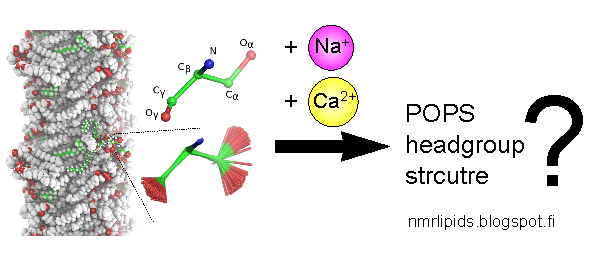
\includegraphics[width=8.5cm]{../Figs/TOC_graphic.pdf}
\end{tocentry}


\begin{abstract}
Phosphatidylserine (PS) is a negatively
charged lipid type commonly found in eukaryotic membranes, where it interacts with proteins via
nonspecific electrostatic interactions as well as via specific binding. Moreover, in the presence of calcium ions, PS lipids can induce
membrane fusion and phase separation.
Molecular details of these phenomena remain poorly understood, partly
because accurate models to interpret the experimental data have not
been available. Here we
gather a set of previously published experimental NMR data of C--H bond order parameter magnitudes, $|S_\mathrm{CH}|$, for pure
PS and mixed PS:PC (phosphatidylcholine) lipid bilayers, 
and augment this data set by measuring the signs of $S_\mathrm{CH}$ in the PS headgroup using S-DROSS solid-state NMR spectroscopy.
The augmented data set is then used
to assess the accuracy of the PS headgroup structures in, and the cation binding to, PS-containing membranes
in the most commonly used classical molecular dynamics (MD) force fields including CHARMM36, Lipid17, MacRog, Slipids, GROMOS-CKP, Berger, and variants.
We show large discrepancies between different force fields, and that none of them reproduces the NMR data within experimental accuracy.
However, the best MD models can detect the most essential differences between PC and PS headgroup structures.
The cation binding affinity is, in line with our previous results for PC lipids, not captured correctly by any of the PS force fields.
Moreover, the simulated response of PS headgroup to bound ions can differ from experiments even \emph{qualitatively}. The collected experimental dataset and simulation
results will pave the way for development of lipid force fields that correctly
describe the biologically relevant negatively charged membranes and their interactions with ions.
This work is part of the NMRlipids open collaboration project (\url{nmrlipids.blogspot.fi}).
\end{abstract}

%\pacs{}% insert suggested PACS numbers in braces on next line

\maketitle %\maketitle must follow title, authors, abstract and \pacs

\section{Introduction}
Phosphatidylserine (PS) is the most common negatively
charged lipid type in eukaryotic biomembranes. In red blood cells, for example,
PS lipids compose 8.5\% of the total lipid weight~\cite{lemmon08}. 
The abundance, however, varies between different cells and organelles, and up to
25--35\% of the cytosolic leaflet of plasma membranes consists of PS lipids~\cite{leventis10,li14}.
PS lipids are vastly important biomolecules that interact with
signaling proteins \cite{leventis10}, regulate
surface charge and protein localization \cite{yeung08}, and
induce protein aggregation \cite{zhao04,gorbenko06}.
Some protein domains interact specifically with PS lipids,
while other protein sites attract PS lipids by nonspecific electrostatics and the
binding can be regulated by calcium \cite{leventis10}.
Therefore, deciphering the structural details
of lipid headgroups and the details of cation binding
is crucial for understanding PS-mediated processes on cellular membranes.

Experimental studies have indicated that the
serine headgroup in PS is more rigid than the choline headgroup in phosphatidylcholine (PC),
owing possibly to electrostatic interactions or formation of a hydrogen bond network between the headgroups~\cite{browning80,buldt81}.
While most monovalent ions interact weakly with
PS-containing bilayers, multivalent cations and Li$^+$ are able to form strong
dehydrated molecular complexes with PS lipids \cite{hauser77,kurland79,eisenberg79,hauser83,dluhy83,hauser85,feigenson86,mattai89,roux90,roux91,boettcher11}.
The dehydrated complexes of PS headgroups with calcium ions can even lead to
phase separation \cite{hauser77,kurland79,hauser85,feigenson86,mattai89,roux90,roux91}. Mixing PS lipids with PC lipids reduces their propensity to form strong complexes with multivalent ions and makes the PS headgroup less rigid~\cite{browning80,buldt81,roux90,roux91}.
That being said, some studies suggest that Ca$^{2+}$ has similar specific binding affinity 
to both negatively charged and zwitterionic phospholipids, and that
the increased cation binding to PS lipid bilayers is non-specific and arises only due to the increased local cation concentration in the vicinity of the membrane~\cite{seelig90,sinn06}. 



Molecular level interpretations of the rigidity of PS headgroup and its interactions with ions
are currently lacking. Classical molecular dynamics (MD) simulations have been widely used in efforts 
to understand the PS headgroup structure, its influence on lipid bilayer properties, and its
interaction with
ions \cite{cascales96,pandit02,mukhopadhyay04,pedersen06,vernier09,boettcher11,molina12,jurkiewicz12,venable13,pan14,vangaveti14,melcrova16,valentine18,hallock18}.
Unfortunately, the results have depended on the particular force field used.
For example, recent simulations using the NBfix parameters for Ca$^{2+}$~\cite{kim16} in
the CHARMM36 force field \cite{klauda10,venable13}, combined with 2D infrared spectroscopy,
suggest that calcium ions interact only with the carboxylate group of PS lipids \cite{valentine18}. In contrast,
the results from the same lipid model without the NBfix ion parameters, combined with NMR chemical shifts and
rotational-echo double-resonance (REDOR) experiments, indicate a significant binding affinity also toward the phosphate region \cite{hallock18}.
Meanwhile, simulations with the Berger force field \cite{berger97,mukhopadhyay04},
combined with fluorescent and vibrational sum frequency spectroscopy, suggest substantial
calcium binding to the carbonyls in the acyl chains \cite{melcrova16}.

We have recently demonstrated that the lipid C--H bond order parameters, $S_\mathrm{CH}$,
can be used to resolve such controversies~\cite{botan15,catte16}. The $S_\mathrm{CH}$ can be
measured from NMR experiments with high accuracy and directly compared to simulations
to either evaluate the quality of the simulation model and/or to interpret the experiments \cite{ollila16}. Using this approach,
it has been established that the structure of PC lipid headgroup and glycerol backbone are not well
captured by most MD force fields~\cite{botan15}, that the cation binding to PC
lipid bilayers is overestimated~\cite{catte16}, and that the inequivalent order parameters of the distinct C--H bonds at
carbon 2 in {\it sn}-2 lipid tails is correctly reproduced only in the CHARMM36 force field~\cite{piggot17}.

Here, we first extend the available set of experimentally measured PS lipid headgroup and
glycerol backbone C--H bond order parameters
by measuring the signs of these order parameters using S-DROSS solid-state NMR spectroscopy.
Based on the collected experimental data, we then assess
the quality of headgroup structures and the ion binding affinity in
the available MD simulation models of PS lipids.
Our results pave the way
for the development of lipid models that correctly describe 
the headgroup region of negatively charged lipids under physiological salt
conditions. Such force fields are expected to be extremely useful in understanding
the biological functions of lipid headgroups and glycerol backbone, as
these are known to behave similarly in simple model membranes and in cells \cite{gally81,scherer87,seelig90}.


\section{Methods}

\subsection{Experimental C--H bond order parameters}

The magnitudes of headgroup and glycerol backbone C--H bond order parameters of 1-palmitoyl-2-oleoyl-{\it sn}-glycero-3-phospho-L-serine (POPS)
were determined by measuring the chemical-shift resolved dipolar splittings
with a R-type Proton Detected Local Field (R-PDLF) experiment~\cite{dvinskikh04}.
The corresponding order parameter signs were measured with a S-DROSS experiment~\cite{gross97}
using natural abundance $^{13}$C solid state NMR spectroscopy as described previously \cite{ferreira13,ferreira16}.
The experiments were done in a Bruker Avance III 400 spectrometer operating at a $^1$H Larmor frequency of 400.03~MHz.
Magic angle spinning (MAS) of the sample was used at a frequency of 5.15~kHz (R-PDLF) and 5~kHz (S-DROSS).
The following experimental setups were used.

{\emph{C--H bond order parameters from the R-PDLF experiment.}} The parameters are described according to Figures 1c and 2c of the original reference
for the R-PDLF experiment~\cite{dvinskikh04}.  The refocused-INEPT delays were $\tau_1=1.94$~ms and $\tau_2=0.97$~ms.
The used radio frequency pulses had the following nutation frequencies: 46.35~kHz (R18$^7_1$ pulses), 63.45~kHz ($^{13}$C 90$^{\circ}$ and 180$^{\circ}$),
50~kHz (SPINAL64 $^1$H decoupling pulses).
The $t_1$ increment was equal to 10.79~$\mu$s $\times18\times2$, and 32 points in the indirect
dimension were recorded using 1024 scans for each, with a recycle delay of 5~s and a spectral width of 149.5~ppm.

\emph{Order parameter signs from the S-DROSS experiment.}
The parameters are described according to Figures 1b and 1c of the original reference for the S-DROSS
experiment~\cite{gross97}. The refocused-INEPT delay $\delta_2$ was 1.19~ms. The $\tau_1$ and $\tau_2$ in the S-DROSS recoupling
blocks $R$ were set as $\tau_1=39.4$~$\mu$s and $\tau_2=89.4$~$\mu$s. The used radio frequency pulses had the nutation
frequencies: 63.45~kHz ($^{13}$C 90$^{\circ}$ and 180$^{\circ}$), 50~kHz ($^1$H\,SPINAL64 decoupling).
The $t_1$ increment (dipolar recoupling dimension) was 800~$\mu$s, and a total of 8 points along $t_1$ were
measured using 1024 scans for each, with a recycle delay of 5~s and a spectral width of 149.5~ppm.

\emph{Numerical simulations of S-DROSS curves.}
The numerical simulations of S-DROSS curves were performed using the SIMPSON simulation package \cite{bak00}
by inputing the $^{13}$C--$^1$H
dipolar couplings, either as determined by the R-PDLF experiments, or as calculated from the known $^2$H quadrupolar couplings \cite{browning80}.
The chemical shift anisotropy and homonuclear couplings were neglected, and the SIMPSON input file {\it{rep2000}} was used to simulate a random
distribution of bilayer orientations in the samples studied.

\emph{Sample preparation.}
The sample was prepared simply by mixing POPS powder (1-palmitoyl-2-oleoyl-{\it sn}-glycero-3-phospho-L-serine, purchased from Avanti Polar Lipids
as sodium salt) with water (lipid:water 60:40~wt-\%) in an Eppendorf tube, centrifuging the mixture and stirring with a thin glass rod repeatedly (approximately 5 to 6 times centrifuging/stirring) until a homogeneous viscous fluid was visually observed. Then 20 mg of the sample was transferred to an NMR insert suitable for 4~mm NMR rotors.  


\subsection{Molecular dynamics simulations}
Molecular dynamics simulation data were collected using
the Open Collaboration method \cite{botan15}, with
the NMR\-lipids Project blog (\url{nmrlipids.blogspot.fi}) and
GitHub repository (\url{github.com/NMRlipids/NMRlipidsIVotherHGs})
as the communication platforms.
The simulated systems are listed in 
Tables \ref{PSsystems} (pure PS bilayers without additional ions) 
and \ref{mixedIONsystems} (mixed PC:PS bilayers at various salt concentrations).
Further simulation details are given in the SI, and
the simulation data are indexed in a
searchable database available at \url{www.nmrlipids.fi},
and in the NMRlipids/MATCH repository (\url{github.com/NMRlipids/MATCH})~\cite{MATCHgit}.

%\begin{table*}[htb]
\begin{sidewaystable*}[!p]
\centering
\caption{List of MD simulations of pure PS bilayers without additional salt. 
  Notation 2$\times$[time] indicates that two independent MD runs were conducted.
  JC refers to the Joung--Cheatham ion parameters~\cite{joung08} and ff99 to the default Amber ion parameters~\cite{aqvist90}.
  Additional simulation details are given in the Supporting Information.
  $^*$ Force field parameters for PS lipids generated for this work, for full details see the Supporting Information.
}\label{PSsystems}
%begin{minipage}[t]{\textwidth}
\begin{tabular}{lcrrrrrcc}
%\hline
% some footnotes are not visible in typeset-MS (pdf)
lipid/counter-ions  & force field & \footnote{Number of lipid molecules}N$_{{\rm l}}$  & \footnote{Number of water molecules}N$_{{\rm w}}$  & \footnote{Simulation temperature}T (K)  & \footnote{Total simulation time}t$_{{\rm sim}}$(ns)  & \footnote{Time used for analyses}t$_{{\rm anal}}$ (ns)  & \footnote{Number of reference for simulation files}files & \tabularnewline
\hline 
POPS/Na$^{+}$  & CHARMM36 \cite{venable13}  & 128  & 4480  & 298  & 2$\times$500  & 2$\times$100  & \citenum{charmm36POPS298K}  & \tabularnewline
POPS/K$^{+}$  & CHARMM36 \cite{venable13}  & 128  & 4480  & 298  & 2$\times$500  & 2$\times$100  & \citenum{charmm36POPS298Kpotassium}  & \tabularnewline
POPS/Na$^{+}$  & CHARMM36-UA$^*$ \cite{venable13,lee14} & 128  & 4480  & 298  & 2$\times$500  & 2$\times$100  & \citenum{charmm36uaPOPS298K}  & \tabularnewline
POPS/Na$^{+}$  & MacRog \cite{maciejewski14}  & 128  & 4480  & 298  & 2$\times$500  & 2$\times$100  & \citenum{macrogPOPS298Kcorrect}  & \tabularnewline
POPS/K$^{+}$  & MacRog \cite{maciejewski14}  & 128  & 4480  & 298  & 200  & 150  & \citenum{macrogPOPS298KwithK}  & \tabularnewline
POPS/Na$^{+}$  & Lipid17 \cite{gould18} / JC \cite{joung08}  & 128  & 4480  & 298  & 2$\times$600  & 2$\times$100  & \citenum{lipid17POPSjcions}  & \tabularnewline
POPS/Na$^{+}$  & Lipid17 \cite{gould18} / ff99 \cite{aqvist90}  & 128  & 4480  & 298  & 2$\times$600  & 2$\times$100  & \citenum{lipid17POPSff99ions}  & \tabularnewline
POPS/Na$^{+}$  & Berger \cite{mukhopadhyay04}  & 128  & 4480  & 298  & 2$\times$500  & 2$\times$100  & \citenum{bergerPOPS298K}  & \tabularnewline
POPS/Na$^{+}$  & GROMOS-CKPM \cite{Chandrasekhar03,kukol09,piggot12} & 128  & 4480  & 298  & 2$\times$500  & 2$\times$100  & \citenum{ckp1POPS303K}  & \tabularnewline
POPS/Na$^{+}$  & GROMOS-CKP \cite{Chandrasekhar03,kukol09,piggot12} & 128  & 4480  & 298  & 2$\times$500  & 2$\times$100  & \citenum{ckp2POPS303K}  & \tabularnewline
POPS/Na$^{+}$  & Slipids \cite{jambeck13}  & 128  & 4480  & 298  & 2$\times$500  & 2$\times$100  & \citenum{slipidsPOPS298K}  & \tabularnewline
\hline 
DOPS/Na$^{+}$  & CHARMM36 \cite{venable13}  & 128  & 4480  & 303  & 2$\times$500  & 2$\times$100  & \citenum{charmm36DOPS303K}  & \tabularnewline
DOPS/Na$^{+}$  & CHARMM36-UA$^*$ \cite{venable13,lee14} & 128  & 4480  & 303  & 2$\times$500  & 2$\times$100  & \citenum{charmm36uaDOPS303K}  & \tabularnewline
DOPS/Na$^{+}$  & Lipid17 \cite{gould18} / JC \cite{joung08}  & 128  & 4480  & 303  & 2$\times$600  & 2$\times$100  & \citenum{lipid17DOPSjcions}  & \tabularnewline
DOPS/Na$^{+}$  & Lipid17 \cite{gould18} / ff99 \cite{aqvist90}  & 128  & 4480  & 303  & 2$\times$600  & 2$\times$100  & \citenum{lipid17DOPSff99ions}  & \tabularnewline
DOPS/Na$^{+}$  & Berger \cite{mukhopadhyay04}  & 128  & 4480  & 303  & 2$\times$500  & 2$\times$100  & \citenum{bergerDOPS303K}  & \tabularnewline
DOPS/Na$^{+}$  & GROMOS-CKPM$^*$ \cite{piggot12} & 128  & 4480  & 303  & 2$\times$500  & 2$\times$100  & \citenum{ckp1DOPS303K}  & \tabularnewline
DOPS/Na$^{+}$  & GROMOS-CKP$^*$ \cite{piggot12}  & 128  & 4480  & 303  & 2$\times$500  & 2$\times$100  & \citenum{ckp2DOPS303K}  & \tabularnewline
DOPS/Na$^{+}$  & Slipids \cite{jambeck13}  & 128  & 4480  & 303  & 2$\times$500  & 2$\times$100  & \citenum{slipidsDOPS303K}  & \tabularnewline
DOPS/Na$^{+}$  & Slipids \cite{jambeck13}  & 288  & 11232  & 303  & 200  & 100  & \citenum{slipidsDOPSfiles}  & \tabularnewline
\end{tabular}
%\end{minipage}
\end{sidewaystable*} 
%\end{table*}




%\begin{table*}[tb]
\begin{sidewaystable*}[!p]
\vspace{1cm}
  \centering
\caption{List of POPC:POPS mixtures simulated at different molar fractions and different amounts of added CaCl$_2$. 
  The salt concentrations are calculated as [salt]=N$_{\rm c} \times$[water]\,/\,N$_{\rm w}$, where [water]\,=\,55.5~M.
  This corresponds to the concentrations in buffer before solvating lipids, which were
  reported in the experiments by Roux et al.~\cite{roux90}.
  Notation 2$\times$[time] indicates that two independent MD runs were conducted.
  Dang refers to the ion parameters by Dang and co-workers~\cite{smith94,dang06}, and ff99 to the default Amber ion parameters~\cite{aqvist90}.
  Additional simulation details are given in the Supporting Information.
  Symbols have the same meaning as in Table \ref{PSsystems}.
}\label{mixedIONsystems}
%begin{minipage}[t]{\textwidth}
\resizebox{0.87\textwidth}{!}{\begin{tabular}{lccccccccc}
  %lipid/counter-ions  & force field & {[}CaCl$_{2}${]}\,(M)  & \footnote{Number of POPC molecules}N$_{{\rm l}}$  & \footnote{Number of water molecules}N$_{{\rm w}}$  & \footnote{Number of Ca$^{2+}$ cations in addition to counter ions}N$_{{\rm c}}$  & \footnote{Simulation temperature}T (K)  & \footnote{Total simulation time}t$_{{\rm sim}}$(ns)  & \footnote{Time used for analyses}t$_{{\rm anal}}$ (ns)  & \footnote{Reference for simulation files}files\tabularnewline
  lipids/counter-ion  & force field & {\footnote{For systems with Ca$^{2+}$ counterions this column gives [Ca$^{2+}$].}[}CaCl$_{2}${]}\,(M)  & N$_{{\rm l}}$  & N$_{{\rm w}}$  & \footnote{Number of Ca$^{2+}$ cations in the system}N$_{{\rm c}}$  & T (K)  & t$_{{\rm sim}}$(ns)  & t$_{{\rm anal}}$ (ns)  & files\tabularnewline
\hline 
%    POPC:POPS (5:1)/K$^+$  & CHARMM36 \cite{klauda10,venable13} &0  & 110:22 & 4935 & 0  & 298  & 100 & 100 \todoi{Equilibration?} & \cite{charmm36pops+83popcT298K}  \\
POPC:POPS (5:1)/Na$^{+}$  & CHARMM36 \cite{klauda10,venable13}  & 0  & 110:22 & 4620  & 0  & 298  & 2$\times$500  & 2$\times$100  & \citenum{charmm36pops+83popcT298KpiggotSODIUM} \tabularnewline
POPC:POPS (5:1)/K$^{+}$  & CHARMM36 \cite{klauda10,venable13}  & 0  & 110:22  & 4620  & 0  & 298  & 2$\times$500  & 2$\times$100  & \citenum{charmm36pops+83popcT298Kpiggot} \tabularnewline
POPC:POPS (5:1)/K$^{+}$  & CHARMM36 \cite{klauda10,venable13}  & 0  & 250:50  & 11207  & 0  & 298  & 200  & 180  & \citenum{POPC5POPS1noCaClCHARMM} \tabularnewline
POPC:POPS (5:1)/Ca$^{2+}$  & CHARMM36 \cite{klauda10,venable13} / NBfix1 \cite{kim16}  & 0.26  & 250:50 & 11190  & 53  & 298  & 200  & 180  & \citenum{POPC5POPS1withCaClCHARMM} \tabularnewline
POPC:POPS (5:1)/Ca$^{2+}$  & CHARMM36 \cite{klauda10,venable13} / NBfix1 \cite{kim16}  & 1.06  & 250:50 & 11174  & 214  & 298  & 200  & 180  & \citenum{POPC5POPS1with1MCaClCHARMM} \tabularnewline
POPC:POPS (5:1)/Na$^{+}$  & CHARMM36 \cite{klauda10,venable13}  & 0  & 250:50  & 11207  & 0  & 320  & 400  & 300  & \citenum{POPC5POPS1CHARMMwithNBfixHan} \tabularnewline
POPC:POPS (5:1)/Na$^{+}$  & CHARMM36 \cite{klauda10,venable13} / NBfix2 \cite{han2018graph}  & 0.14  & 250:50 & 11190  & 28  & 320  & 440  & 300  & \citenum{POPC5POPS1CHARMMwithNBfixHan} \tabularnewline
POPC:POPS (5:1)/Na$^{+}$  & CHARMM36 \cite{klauda10,venable13} / NBfix2 \cite{han2018graph}  & 0.94  & 250:50 & 11174  & 189  & 320  & 440  & 300  & \citenum{POPC5POPS1CHARMMwithNBfixHan} \tabularnewline
POPC:POPS (1:1)/K$^{+}$  & CHARMM36 \cite{klauda10,venable13}  & 0  & 150:150  & 10785  & 0  & 298  & 200  & 180  & \citenum{POPC1POPS1noCaClCHARMM} \tabularnewline
\hline 
POPC:POPS (1:0)  & MacRog \cite{maciejewski14}  & 0  & 120:0 & 5120  & 0  & 298  & 200  & 150  & \citenum{macrogPOPC298K} \tabularnewline
POPC:POPS (5:1)/K$^{+}$  & MacRog \cite{maciejewski14}  & 0  & 120:24 & 5760  & 0  & 298  & 400 & 250 &  \citenum{POPCpopsMACROG}\tabularnewline
POPC:POPS (5:1)/K$^{+}$  & MacRog \cite{maciejewski14}  & 0.10  & 120:24  & 5760  & 10  & 298  & 600  & 300  & \citenum{POPCpopsMACROG} \tabularnewline
POPC:POPS (5:1)/K$^{+}$  & MacRog \cite{maciejewski14}  & 0.30  & 120:24  & 5760  & 31  & 298  & 600  & 300  & \citenum{POPCpopsMACROG} \tabularnewline
POPC:POPS (5:1)/K$^{+}$  & MacRog \cite{maciejewski14}  & 1.00  & 120:24 & 5760  & 104  & 298  & 600  & 300  & \citenum{POPCpopsMACROG} \tabularnewline
POPC:POPS (5:1)/K$^{+}$  & MacRog \cite{maciejewski14}  & 3.00  & 120:24 & 5760  & 311  & 298  & 600 & 300 & \citenum{POPCpopsMACROG}\tabularnewline
\hline 
%    POPC:OPPS (5:1)/K$^+$  & MacRog \cite{maciejewski14} &4.00    & 0   & 120:24 & 5760 & 415  & 298  & 300 & 200 & \cite{POPCpopsMACROGwithK}  \\
POPC:POPS (5:1)/K$^{+}$  & Lipid14/17 \cite{dickson14,gould18} / ff99~\cite{aqvist90}  & 0  & 120:24  & 5760  & 0  & 298  & 2$\times$500  & 2$\times$200  & \citenum{POPCpopsLIPID17withKCI} \tabularnewline
POPC:POPS (5:1)/Na$^{+}$  & Lipid14/17 \cite{dickson14,gould18} / ff99~\cite{aqvist90}  & 0  & 120:24 & 5760  & 0  & 298  & 2$\times$500  & 2$\times$200  & \citenum{POPCpopsLIPID17withNaCI} \tabularnewline
POPC:POPS (5:1)/Ca$^{2+}$  & Lipid14/17 \cite{dickson14,gould18} / ff99~\cite{aqvist90}  & 0.50  & 120:24 & 5760  & 52  & 298  & 2$\times$500  & 2$\times$200  & \citenum{POPCpopsLIPID17withCaCl} \tabularnewline
POPC:POPS (5:1)/Ca$^{2+}$  & Lipid14/17 \cite{dickson14,gould18} / ff99~\cite{aqvist90}  & 1.00  & 120:24  & 5760  & 104  & 298  & 2$\times$500  & 2$\times$200  & \citenum{POPCpopsLIPID17withCaCl} \tabularnewline
POPC:POPS (5:1)/Ca$^{2+}$  & Lipid14/17 \cite{dickson14,gould18} / ff99~\cite{aqvist90}  & 2.00  & 120:24  & 5760  & 208  & 298  & 2$\times$500  & 2$\times$200  & \citenum{POPCpopsLIPID17withCaCl} \tabularnewline
POPC:POPS (5:1)/Ca$^{2+}$  & Lipid14/17 \cite{dickson14,gould18} / ff99~\cite{aqvist90}  & 3.00  & 120:24 & 5760  & 311  & 298  & 2$\times$500  & 2$\times$200  & \citenum{POPCpopsLIPID17withCaCl} \tabularnewline
POPC:POPS (5:1)/Ca$^{2+}$  & Lipid14/17 \cite{dickson14,gould18} / ff99~\cite{aqvist90}  & 4.00  & 120:24  & 5760  & 415  & 298  & 2$\times$500  & 2$\times$200  & \citenum{POPCpopsLIPID17withCaCl} \tabularnewline
POPC:POPS (5:1)/Na$^{+}$  & Lipid14/17 \cite{dickson14,gould18} / Dang~\cite{smith94,dang06}  & 0  & 60:12 & 3600  & 0  & 298  & 1050  & 1000  & \citenum{lipid17_cacl_series} \tabularnewline
POPC:POPS (5:1)/Na$^{+}$  & Lipid14/17 \cite{dickson14,gould18} / Dang~\cite{smith94,dang06}  & 0.08  & 60:12  & 3561  & 5  & 298  & 1050  & 1000  & \citenum{lipid17_cacl_series} \tabularnewline
POPC:POPS (5:1)/Na$^{+}$  & Lipid14/17 \cite{dickson14,gould18} / Dang~\cite{smith94,dang06}  & 0.13  & 60:12  & 3561  & 8  & 298  & 1050  & 1000  & \citenum{lipid17_cacl_series} \tabularnewline
POPC:POPS (5:1)/Na$^{+}$  & Lipid14/17 \cite{dickson14,gould18} / Dang~\cite{smith94,dang06}  & 0.20  & 60:12 & 3561  & 13  & 298  & 1050  & 1000  & \citenum{lipid17_cacl_series} \tabularnewline
POPC:POPS (5:1)/Na$^{+}$  & Lipid14/17 \cite{dickson14,gould18} / Dang~\cite{smith94,dang06}  & 0.41  & 60:12 & 3522  & 26  & 298  & 1050  & 1000  & \citenum{lipid17_cacl_series} \tabularnewline
POPC:POPS (5:1)/Na$^{+}$  & Lipid14/17 \cite{dickson14,gould18} / Dang~\cite{smith94,dang06}  & 0.62  & 60:12 & 3483  & 39  & 298  & 1050  & 1000  & \citenum{lipid17_cacl_series} \tabularnewline
\hline 
POPC:POPS (4:1)/Na$^{+}$  & Berger \cite{tieleman99,mukhopadhyay04}  & 0  & 102:26 & 4290  & 0  & 310  & 120  & 80  & \citenum{bergerPOPSPOPC4:1mixtureT310K} \tabularnewline
POPC:POPS (4:1)/Ca$^{2+}$  & Berger \cite{tieleman99,mukhopadhyay04}  & 0.102\footnote{\label{noteBerger}Calculation of concentration complicated by the
use of scaled ions. Concentration taken as reported in the delivered
data.}  & 104:26  & 4306  & 24  & 310  & 300  & 100  & \citenum{POPCpopsBERGERwith102mMCa} \tabularnewline
POPC:POPS (4:1)/Ca$^{2+}$  & Berger \cite{tieleman99,mukhopadhyay04}  & 0.715\textsuperscript{\ref{noteBerger}}  & 104:26 & 4306  & 72  & 310  & 300  & 100  & \citenum{POPCpopsBERGERwith715mMCa} \tabularnewline
\hline 
POPC:POPS (5:1)/Na$^{+}$  & GROMOS-CKP\footnote{Force field parameters for PS lipids generated for this work, for full details see the Supporting Information.} \cite{piggot12}  & 0  & 110:22 & 4620  & 0  & 298  & 2$\times$500  & 2$\times$100  & \citenum{POPCpopsGROMOSCKPwithNa} \tabularnewline
POPC:POPS (5:1)/Na$^{+}$  & GROMOS-CKPM$^c$ \cite{piggot12}  & 0  & 110:22 & 4620  & 0  & 298  & 2$\times$500  & 2$\times$100  & \citenum{POPCpopsGROMOSCKPMwithNa} \tabularnewline
\end{tabular}}
%\end{minipage}
\end{sidewaystable*} 
%\end{table*}



The C--H bond order parameters were calculated directly
from the carbon and hydrogen positions using the definition
\begin{equation}
S_{\rm CH}=\frac{1}{2}\langle 3\cos^2\theta -1 \rangle,
\end{equation}
where $\theta$ is the angle between the C--H bond and the membrane normal
(taken to align with $z$, with bilayer periodicity in the $xy$-plane).
Angular brackets denote average over all sampled configurations.
The order parameters were calculated by first averaging over time separately
for each lipid in the system, and then calculating the average and
the standard error of the mean over the different lipids. The analysis can be conducted using a
Python program ({\tt calcOrderParameters.py}, available in Ref.~\citenum{MATCHgit}) that uses the
MDAnalysis library \cite{agrawal11,gowers16}.
For united atom models, the positions of hydrogens were generated before the order parameter calculation using the {\tt protonate} tool
of the Gromacs 3 sofware package \cite{gromacsMANUAL}.
The ion number density profiles were calculated using the {\tt gmx density} tool
of the Gromacs sofware package \cite{gromacsMANUAL}.

\subsection{Using the molecular electrometer concept to compare ion binding to negatively charged lipid bilayers 
in simulations and in experiments}

The $S_{\rm CH}$ of the $\alpha$ and $\beta$ carbons in the PC headgroup
decrease proportionally to the amount of positive
charge bound to the bilayer \cite{akutsu81,altenbach84,seelig87},
and can therefore be used to measure the ion binding affinity.
In addition to ions, the correlation between bound charge and headgroup order parameter change
is empirically observed also for peptides, charged amphiphiles, local anesthetics and charged lipids~\cite{scherer87,beschiaschvili91}.
This concept, known as the molecular electrometer, is especially useful for 
comparison between simulations and experiments, as
the headgroup $S_{\rm CH}$ at varying cation
concentrations can be easily calculated from
simulations~\cite{catte16}. The headgroup $S_{\rm CH}$
of negatively charged PS and PG lipids also exhibit systematic --- although less well understood ---dependencies on the bound charge~\cite{borle85,macdonald87,roux86,roux90}.
Therefore, measuring the PC headgroup $S_{\rm CH}$ from 
mixed (here PS:PC) bilayers~\cite{roux86,roux90,roux91} (see also SI section \ref{electrometerFORmixtures}) provides a more straightforward way of characterizing the ion binding to negatively charged membranes.

Calibrating the PC $S_{\rm CH}$ response to a known amount of bound charge~\cite{catte16,melcr18} is an important preliminary step for using the molecular electrometer.
This can be done using experimental data from mixtures of PC and
monovalent cationic surfactants (such as POPC and dihexadecyldimethylammonium,
see SI section \ref{electrometerCALIBRATION})~\cite{scherer89,melcr18}.
Additionally, the response of PC headgroup $S_{\rm CH}$ to the negatively
charged PS follows the molecular electrometer in experiments~\cite{scherer87},
which we also quantify here (see SI section \ref{electrometerFORmixtures}).

Studies applying the molecular electrometer have used two different definitions for salt concentration:
The concentrations can be reported either before \cite{akutsu81,roux90,catte16}, or after \cite{altenbach84,melcr18} solvating the lipids.
In the former case, binding of ions to the lipids leads to a lower bulk concentration than in what was present in the original solvent.
However, the choice of definition has only a marginal effect
to the results in simulations with realistic ion binding affinity
(see SI section \ref{concentrationDEFsection}).
In this work we use the former definition (concentration before solvating the lipids) to be consistent with the reference
experimental data \cite{roux90}.

\section{Results and Discussion}

\subsection{Headgroup and glycerol backbone C--H bond order parameters of POPS from $^{13}$C NMR}
The INEPT and 2D R-PDLF experiments from POPS samples gave well resolved spectra for all the
carbons in the headgroup and glycerol backbone regions (Fig. \ref{PShgSIGNSsimpson}).
The glycerol backbone carbon peaks were assigned according to the POPC spectra~\cite{ferreira13}, whereas
the peaks for $\beta$ and $\alpha$ carbons were assigned according to the
known C--H bond order parameters from the $^2$H\,NMR experiments~\cite{browning80}.
Slices of the R-PDLF spectra and the resulting  $S_{\rm CH}$ values
are shown in the Supporting Information (Fig. \ref{DPslices}). 

\begin{figure}[!tb]
  \centering
  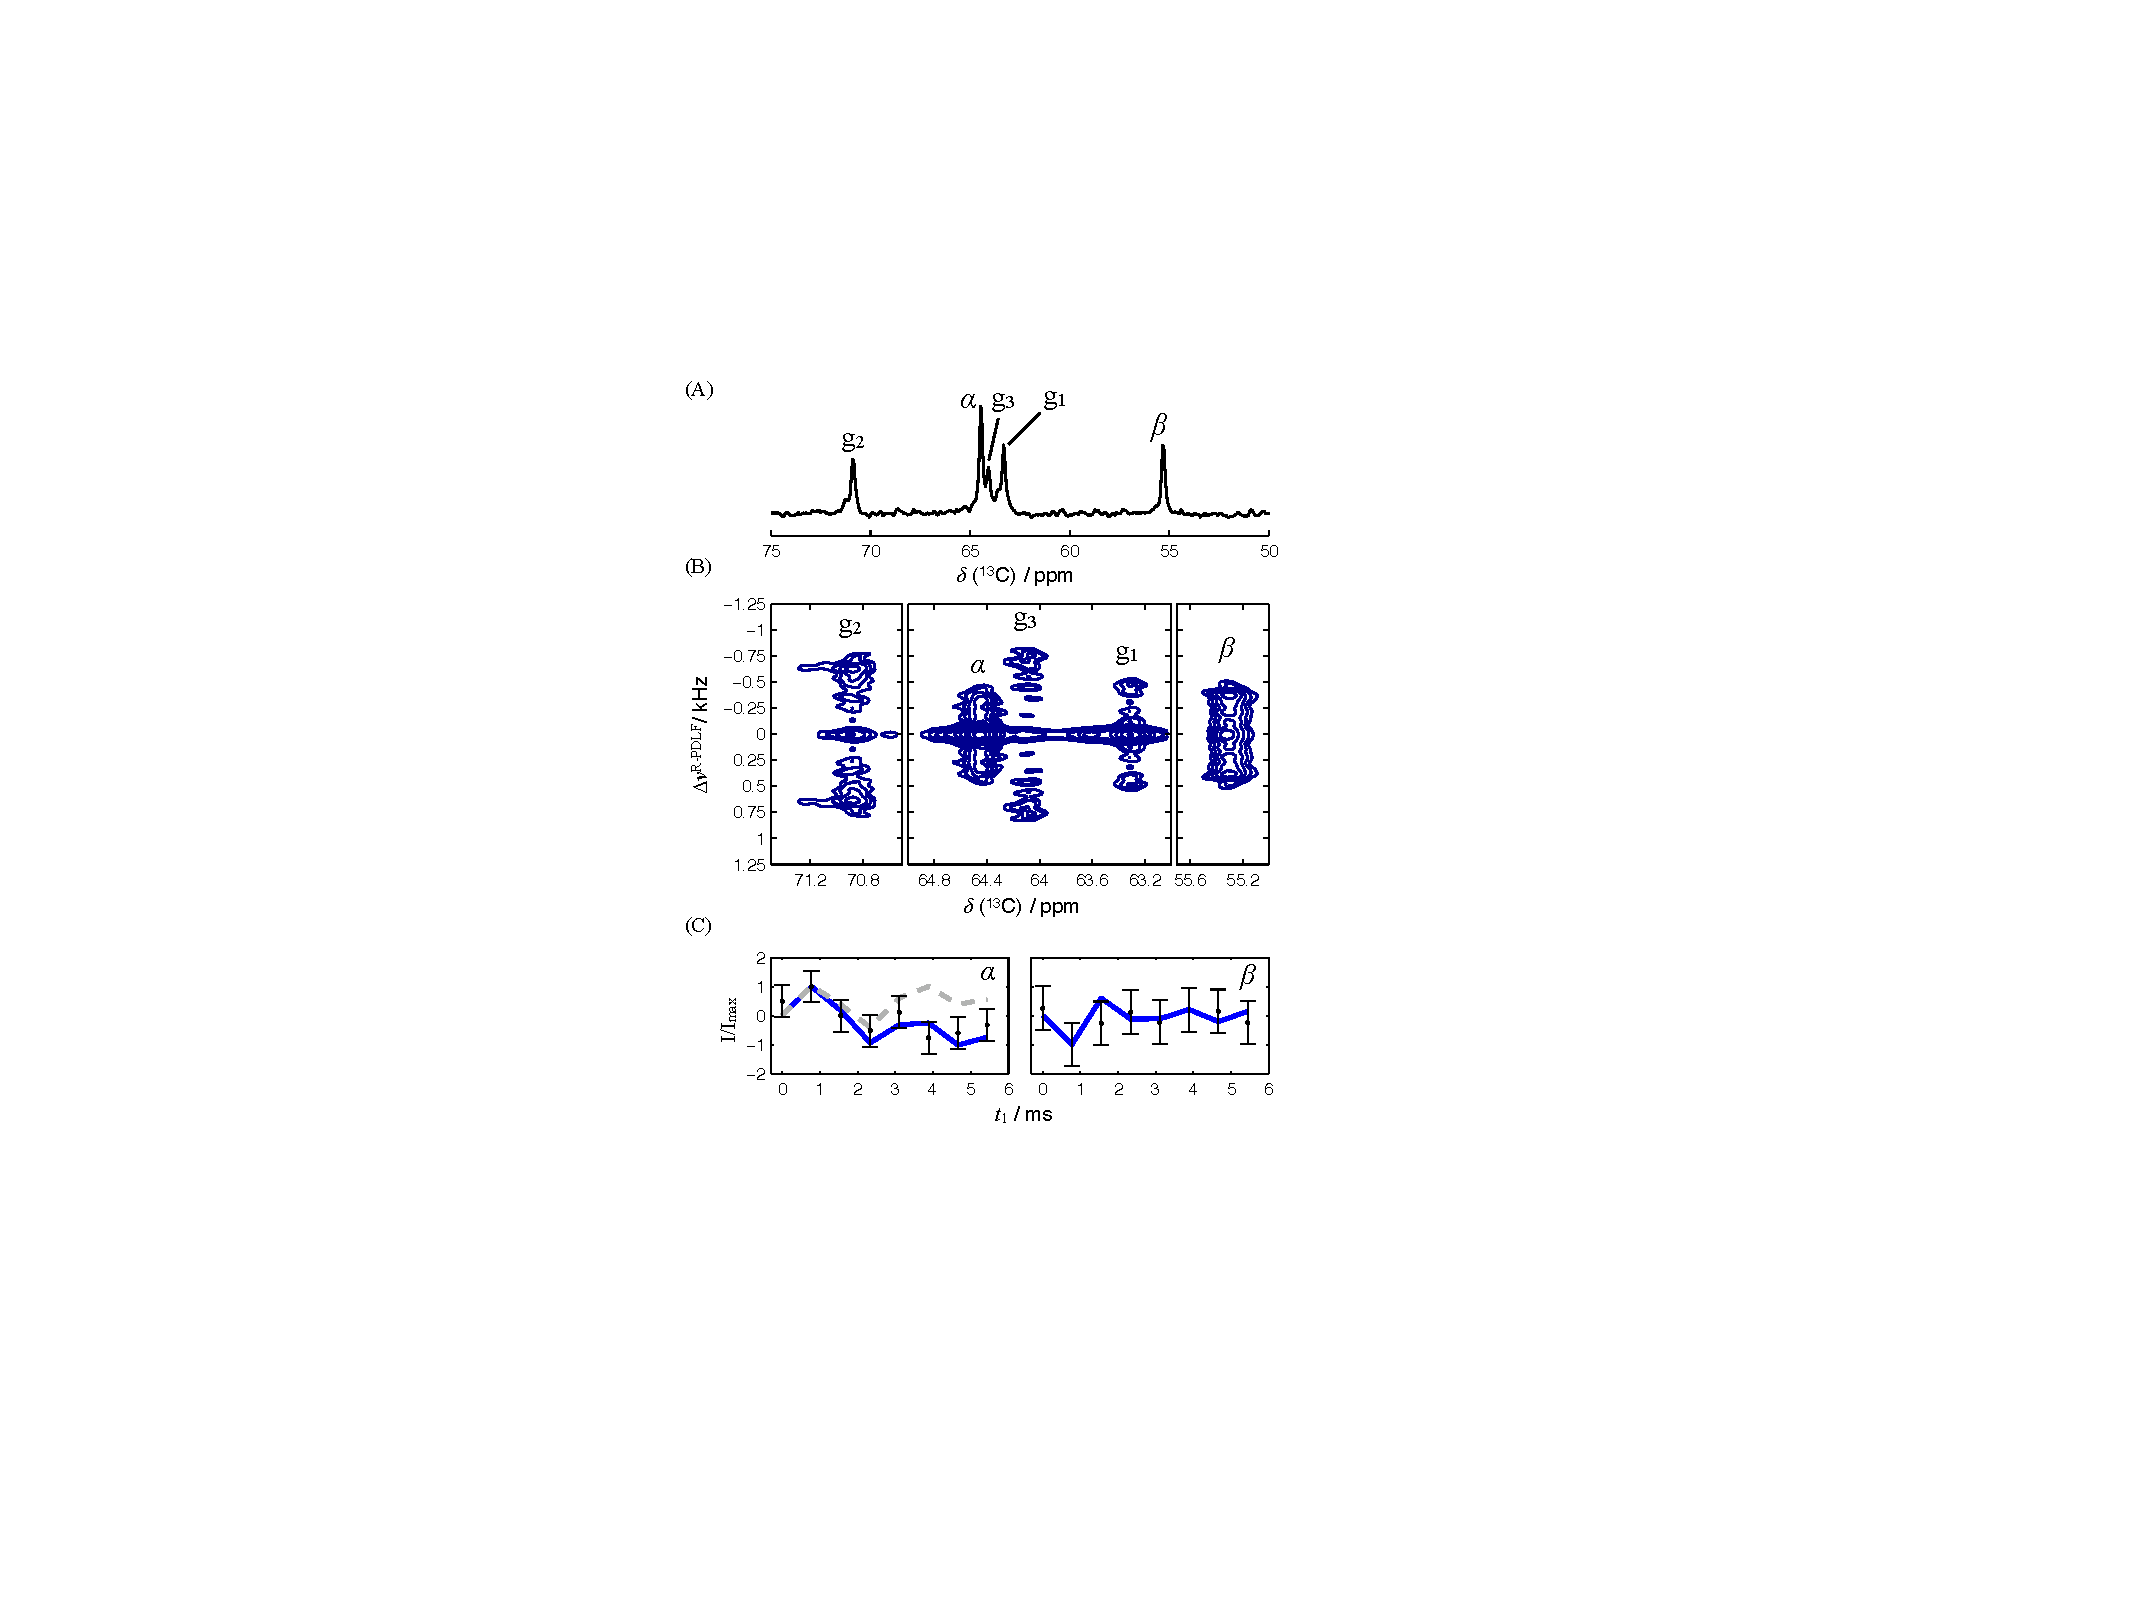
\includegraphics[width=8.5cm]{../Figs/fig1_POPS.pdf}
  \caption{\label{PShgSIGNSsimpson}
    The headgroup and glycerol backbone region of the (A) Refocused-INEPT spectrum and
    (B) 2D R-PDLF spectra.
    (C) Experimental S-DROSS data (points), and SIMPSON simulations (blue lines) with
    the C--H bond order parameter values of $-0.12$ for the $\beta$-carbon, and $+0.09$ and $-0.02$
    for the $\alpha$-carbon.
    Dashed gray line is the S-DROSS curve from a SIMPSON simulation with a positive value ($+0.02$) 
    for the smaller $\alpha$-carbon C--H bond order parameter.
  }
\end{figure}
\begin{figure}[!htb]
  \centering
  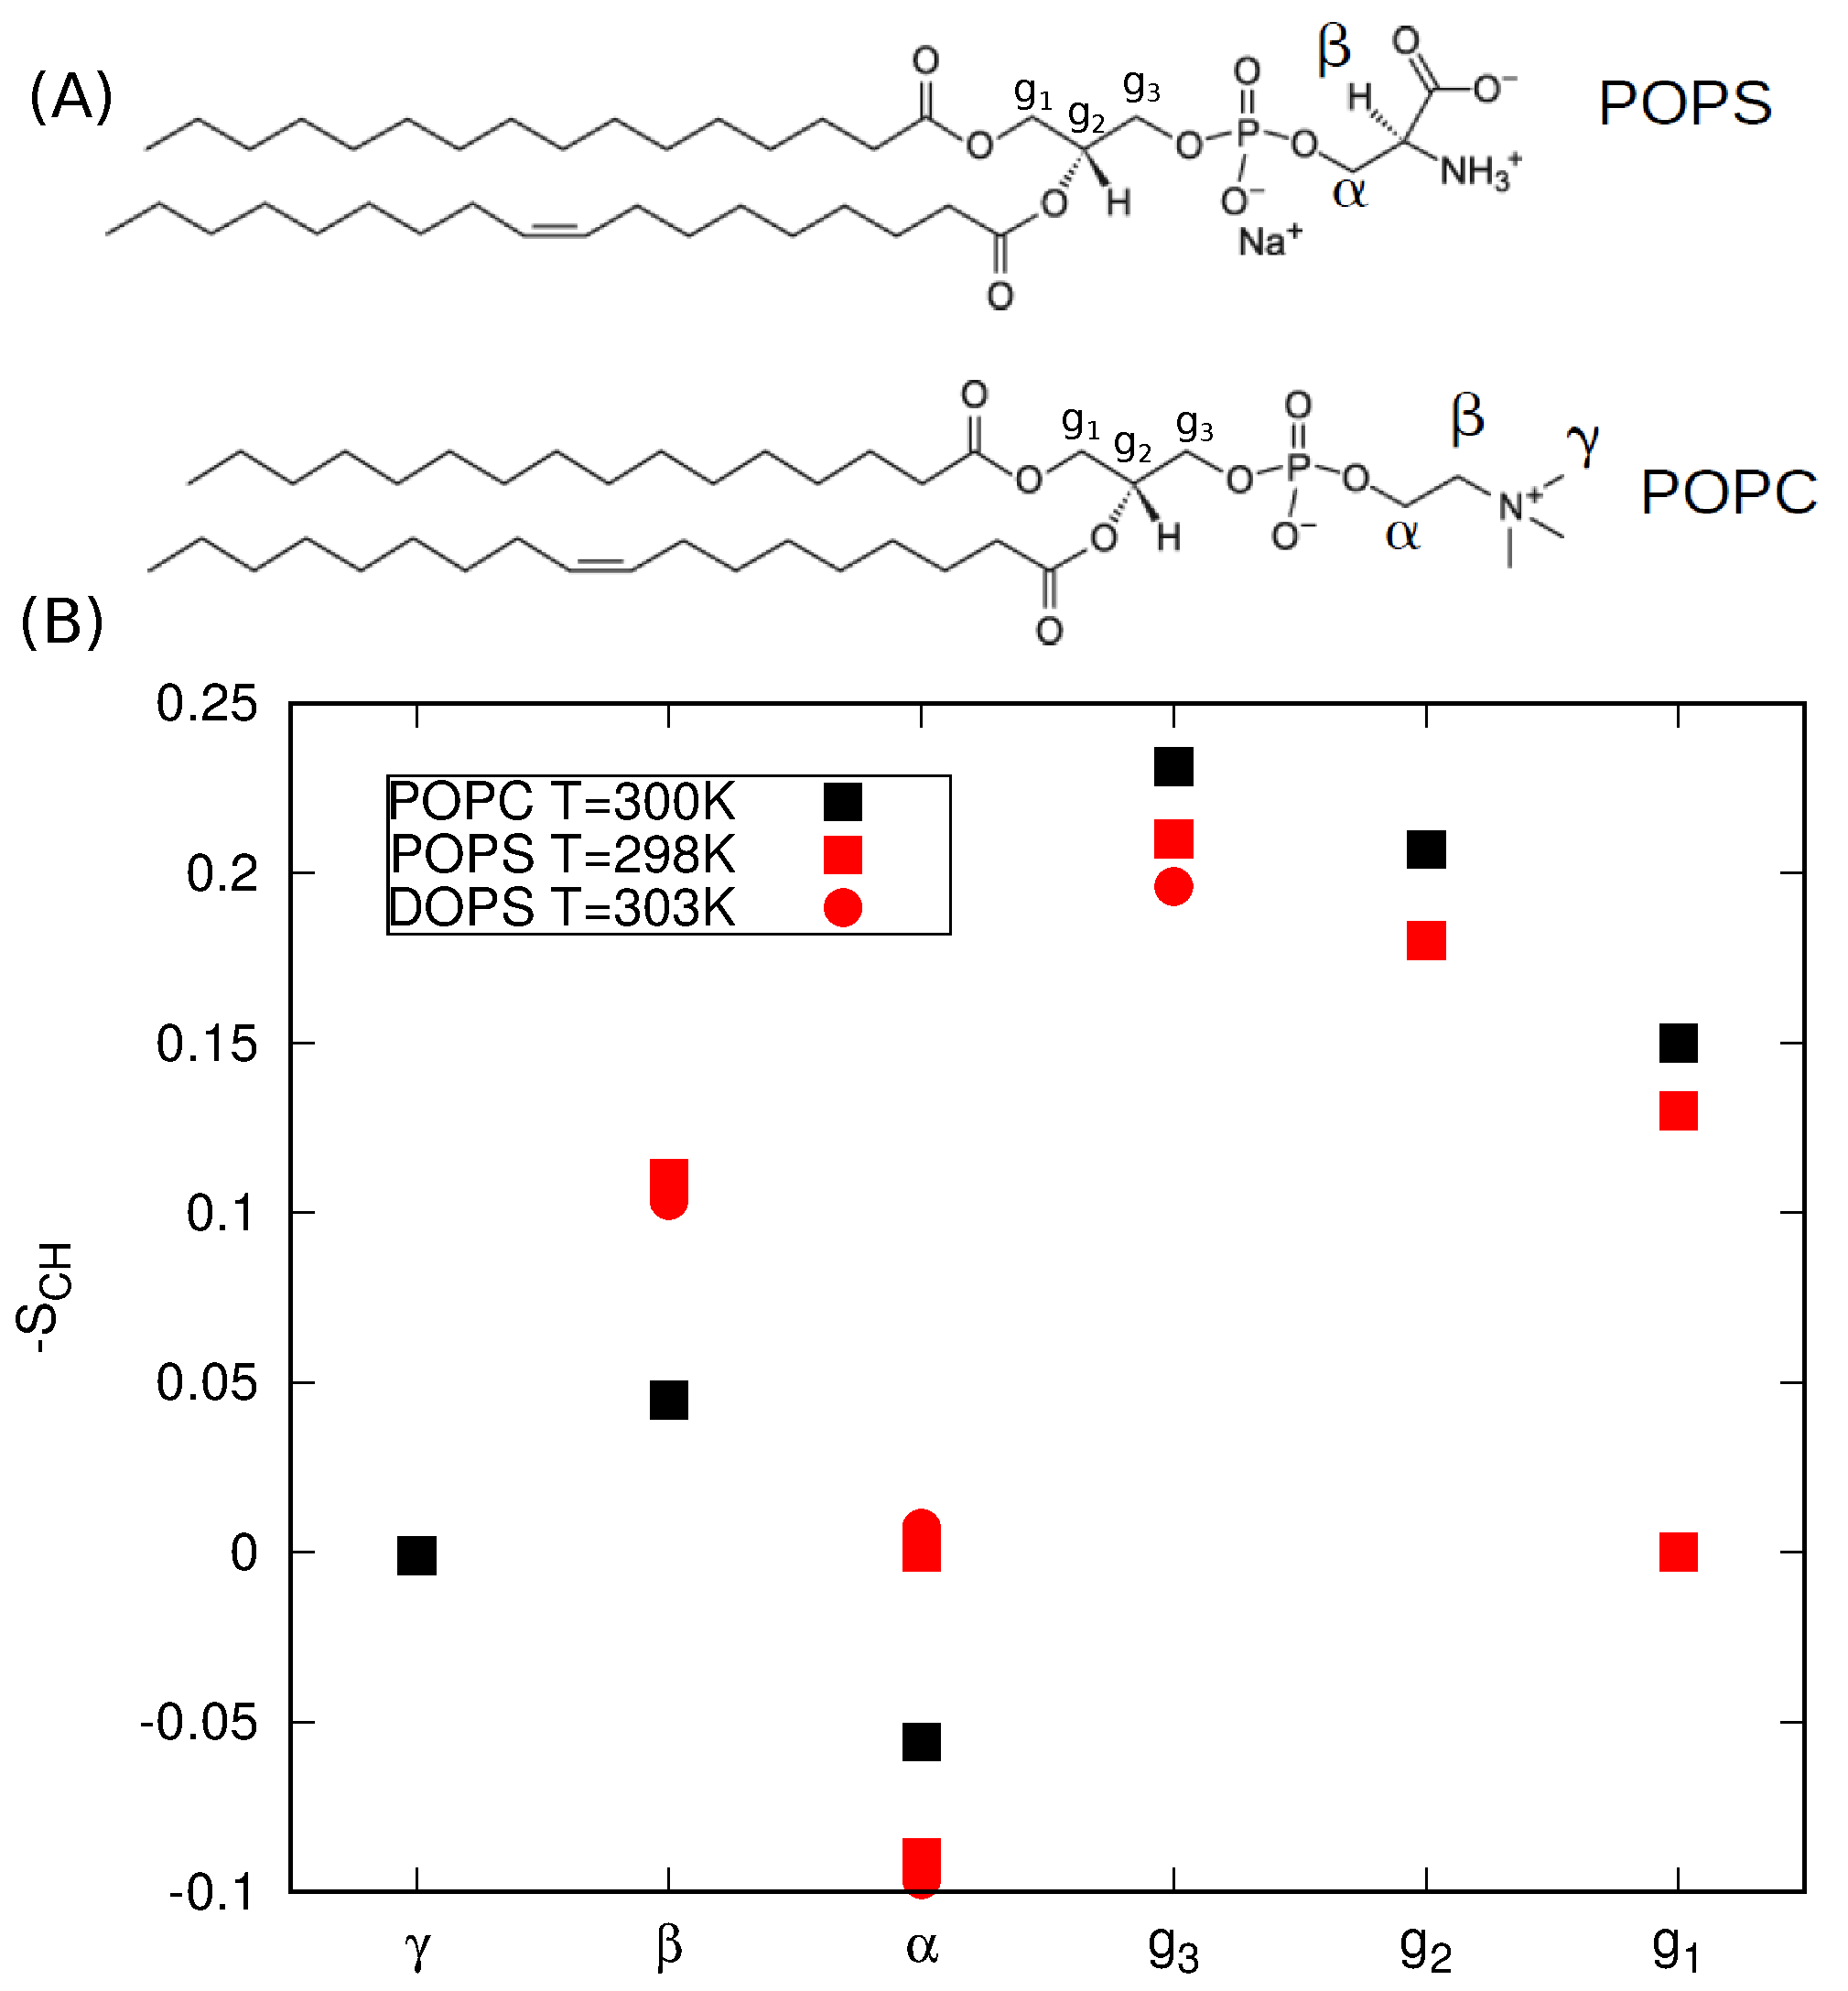
\includegraphics[width=9.0cm]{../Figs/PCPScomp.eps}
  \caption{\label{HGorderParameters}
    (A) Chemical structures and labels for the headgroup and glycerol backbone carbons.
    (B) Headgroup and glycerol backbone order parameters of POPS (T = 298 K) measured in this work compared
    with the previously published values from DOPS ($T=303$~K, $^2$H NMR, 0.1~M of NaCl) \cite{browning80} and 
    POPC  ($T=300$~K, $^{13}$C NMR) \cite{ferreira13} experiments. Signs of the PS order parameters
    are measured in this work whereas signs of the PC order parameters are measured previously~\cite{ferreira16}.
    The size of errorbars ($\pm$0.02) shown for $^{13}$C NMR data is justified previously~\cite{botan15,ollila16}. 
  }
  %\todo{Replacing the "literature" with "from Ref X" has been suggested  https://github.com/NMRLipids/NMRlipidsIVotherHGs/issues/34.
  %We can do this just before submission when citation numbers will not change anymore.}
  %SAMULI: Maybe better to do in revision stage because citations might still change.
\end{figure}

Since the R-PDLF and previous $^2$H\,NMR experiments \cite{browning80,roux91} give 
only the absolute values of  $S_{\rm CH}$, we determined the signs of the PS headgroup
 $S_{\rm CH}$ using the S-DROSS experiment \cite{gross97}.
For a given carbon, its S-DROSS dipolar modulation profile in the indirect dimension is a superposition
of sinusoidal functions from the possible orientations of crystallites in the sample (or bilayer patches).
We phase corrected the 2D spectrum in the direct dimension such that positive and negative signs for the $S_{\rm CH}$ 
give rise to profiles that initially increase and decrease, respectively.
In practice, we use the known negative sign of the acyl chain carbons as a reference to perform
the phase correction and interpret the distinct initial slopes of the S-DROSS profiles (Fig. \ref{DPslices}). 
The S-DROSS slice for the $\beta$-carbon clearly shows an initial decrease and therefore its order parameter must be negative.
For the $\alpha$-carbon such analysis is not as trivial due to the two inequivalent order parameters of the two distinct C--H bonds.
However, the beginning of its S-DROSS slice suggests that the larger $S_{\rm CH}$ of the $\alpha$-carbon is positive and the
decrease towards negative values at longer $t_1$ suggests that the smaller  $S_{\rm CH}$ is negative.    
This is confirmed by a SIMPSON simulation
using the  $S_{\rm CH}$ values of $+0.09$ from the dipolar coupling measured here (Fig. \ref{DPslices})
and $-0.02$ from the previous $^2$H\,NMR experiment~\cite{roux91}.
We used the literature value for the smaller  $S_{\rm CH}$ , because the
resolution of our R-PDLF experiment was not sufficient to determine the
magnitude of the small value.
The S-DROSS curve from the SIMPSON simulation with a positive value for the smaller  $S_{\rm CH}$ 
(dashed grey in Fig. \ref{PShgSIGNSsimpson} C)) did not agree with the experiment, 
corroborating the interpretation that the smaller  $S_{\rm CH}$  is negative.

The headgroup and glycerol backbone order parameters of 
POPS measured in this work are in good agreement with the previously reported
values from $^2$H\,NMR experiments of DOPS \cite{browning80} (Fig. \ref{HGorderParameters}).
When compared with the previously measured values for POPC \cite{ferreira13} (Fig. \ref{HGorderParameters}),
the $\beta$-carbon  $S_{\rm CH}$ is significantly more negative and $\alpha$-carbon
experiences a substantial forking (different  $S_{\rm CH}$ for the two hydrogens in the same carbon \cite{ollila16}) in the PS headgroup.
These features have been intepreted to arise from a rigid PS headgroup
conformation, stabilized by hydrogen bonds or electrostatic
interactions \cite{browning80,buldt81}, but a detailed structrural interpretation is not
available. 

We note that the DOPS $^2$H~NMR reference data found in the literature~\cite{browning80,roux90} was obtained by first solvating
the lipids with a buffer solution and then centrifuging the sample to a pellet that was used for the measurements. Such samples have a lower lipid concentration
(approximately 10~wt~\% of lipids~\cite{browning80,roux88,roux90}) than 
the gravimetric samples (60~wt~\%) and simulations (approximately 50--60~wt~\%) in this work.
Larger multilamellar repeat distances are expected in the samples with lower lipid
concentrations due to the swelling caused by electrostatic repulsion in pure PS lipid systems~\cite{millman82}.
Yet the PS headgroup  $S_{\rm CH}$  measured from gravimetric samples (POPS) in this work
are in good agreement with the results from centrifuged samples~\cite{browning80}. This, together with the rapid decrease of equilibrium repeat distance with addition of monovalent salt~\cite{millman82,rand89}, indicates that the hydration levels of multilamellae are sufficiently similar in the simulations and reference experiments.

\subsection{Headgroup and glycerol backbone in simulations of PS lipid bilayers without additional ions}

The different PS MD models produced highly varied headgroup and glycerol backbone  $S_{\rm CH}$ (Fig.~\ref{HGorderParametersPS})
and structures (Fig.~\ref{HGandGLYstructuresPS} and section~\ref{Diheds} in the Supporting Information).
As was previously observed for PC lipids \cite{botan15}, also none of the PS models produced a set of  $S_{\rm CH}$ in full quantitative agreement with the experiments.
In fact, the models perform less well for PS than for PC
(Figs.~\ref{HGorderParametersPS} and \ref{comparisonTablePS} vs. Figs.~2 and 4 in Ref.~\citenum{botan15}),
which complicates the interpretation of structural differences between the PC and PS. However, concentrating on the headgroup alone, we see that the best performing models (Slipids, CHARMM36, and CHARMM36-UA) indeed do qualitatively replicate the larger-than-in-PC
forking of the $\alpha$-carbon (these models give forkings of $\sim\!0.01$ or smaller for PC~\cite{botan15} and between $\sim\!0.05$ and $\sim\!0.12$ for PS) that is observed in experiments
(Fig.~\ref{HGorderParameters}).
Additionally, the Slipids force field correctly produces the significantly smaller $\beta$-carbon order parameter
for PS ($S^\beta_{\rm CH}\approx-0.09$, see Fig.~\ref{HGorderParametersPS}) compared to PC ($S^\beta_{\rm CH}\approx-0.03$,~see Fig.~2 in Ref.~\citenum{botan15}),
%Fig. \ref{HGorderParametersPS} vs. Fig. 2 in Ref.~\citenum{botan15})
in line with experiments (Fig. \ref{HGorderParameters}).


\begin{figure}[]
  \centering
  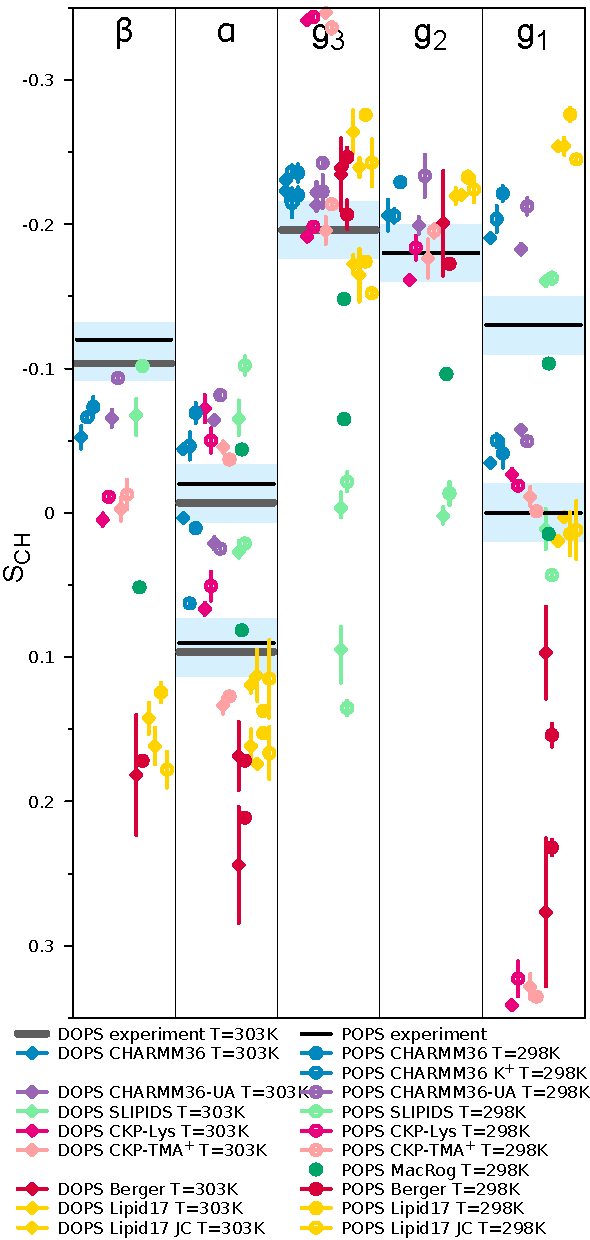
\includegraphics[width=9.0cm]{../Figs/HGorderparametersPS.pdf}
  \caption{\label{HGorderParametersPS}
    C--H bond order parameters, $S_{\rm CH}$, of the PS headgroup ($\beta$ and $\alpha$) and
    glycerol backbone (g$_3$, g$_2$, g$_1$) carbons from NMR experiments (horizontal lines),
    and MD simulations with different force fields (symbols).
    Experimental data for DOPS had been measured with 0.1\,M of NaCl~\cite{browning80},
    while all the other data are with counterions only.
    The data for DOPS is at 303~K and for POPS at 298~K.
    The light blue areas span 0.04 units around the average of the extremal experimental values,
    in accordance with the expected quantitative accuracy of experiments~\cite{ollila16}.
    The vertical bars shown for all simulation values (excl. MacRog~K$^+$)
    are not error bars, but demonstrate that for these systems
    we had at least two data sets; the ends of the bars mark the extreme values
    from the sets, and the symbol marks their measurement-time-weighted average.
  }
\end{figure}

\begin{figure}[]
  \centering
  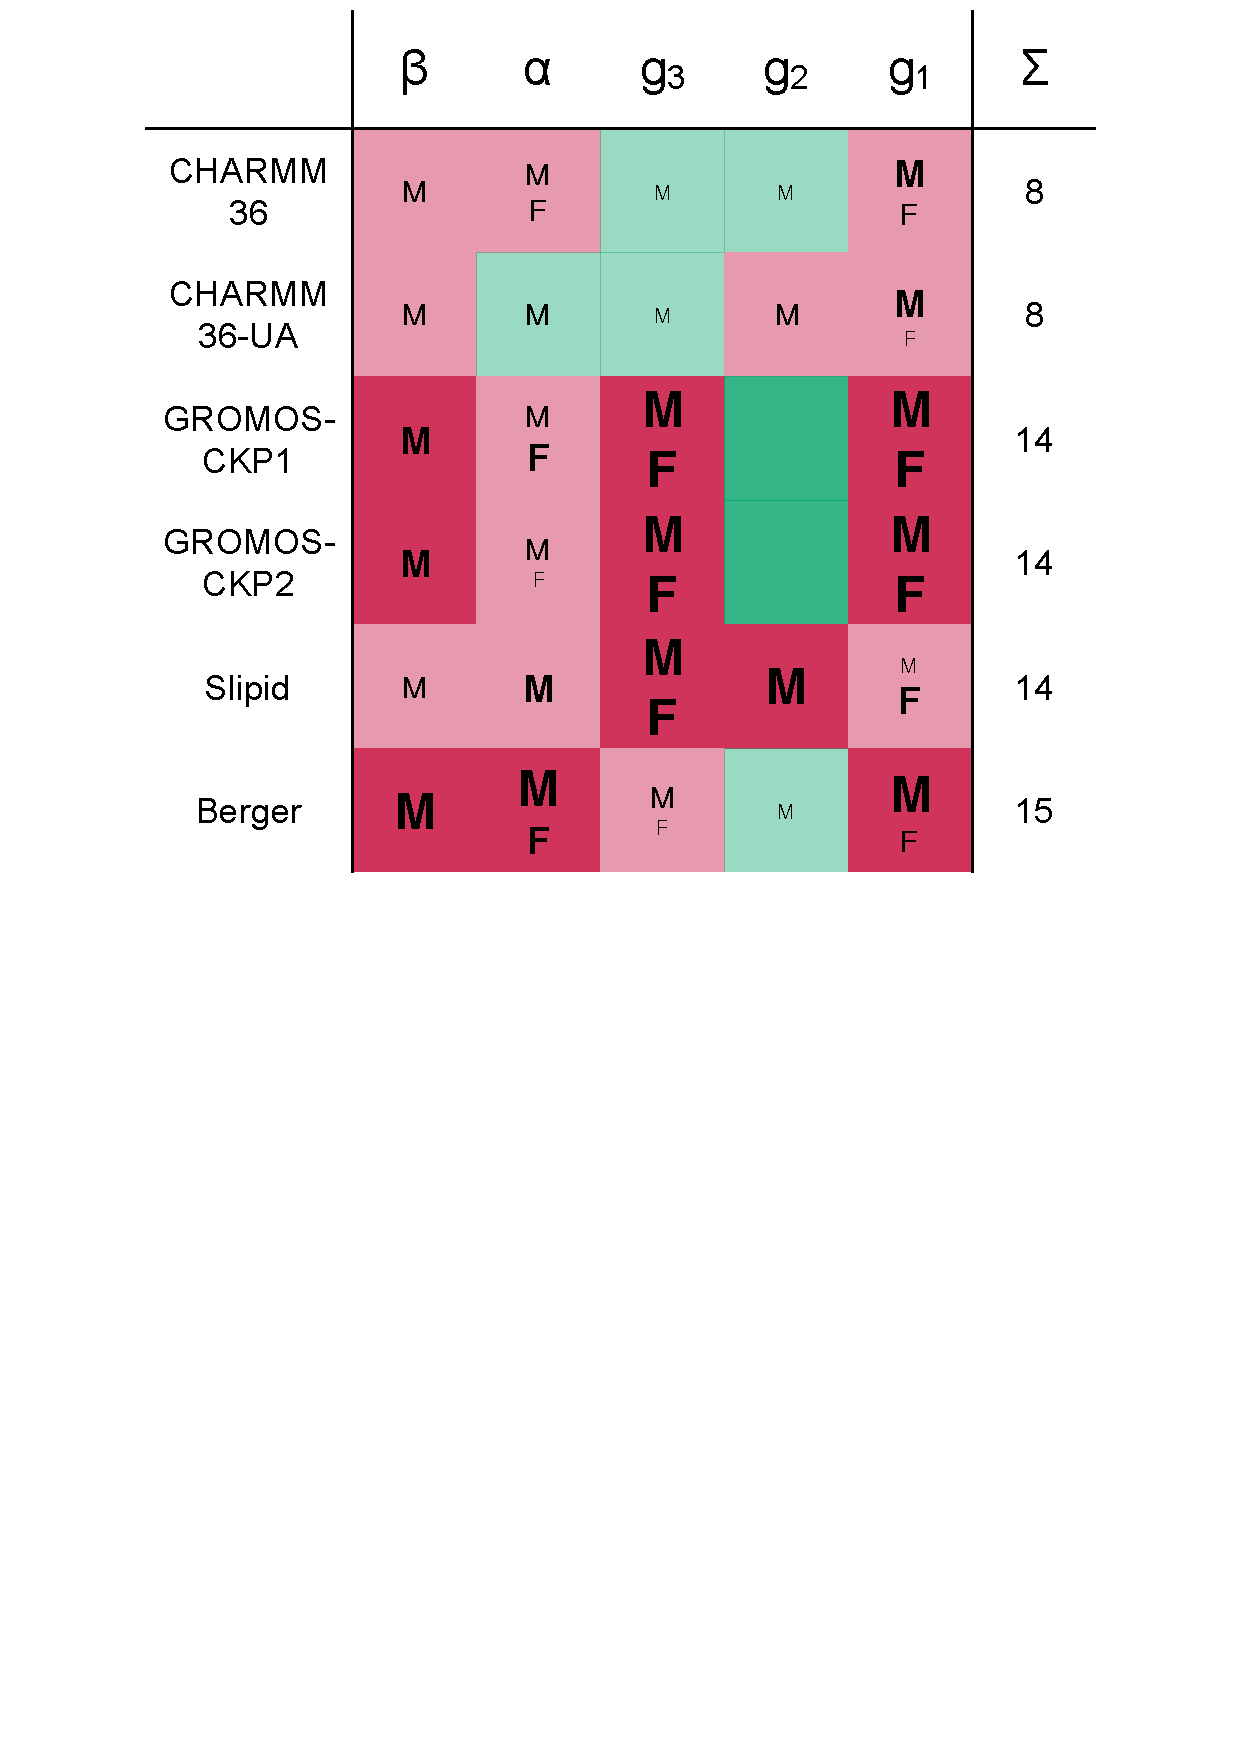
\includegraphics[width=9.0cm]{../Figs/comparisonTablePS.pdf}
  \caption{\label{comparisonTablePS}
    Rough subjective ranking of force fields based on how far the simulated order parameters were from the experimental
    values ({\textsf{\small M}} indicates a magnitude problem) and how well the difference between order parameters
    of two hydrogens attached to the same carbon were reproduced ({\textsf{\small F}} indicates a forking problem)
    in Fig.~\ref{HGorderParametersPS}.
    The letter size increases with problem severity. Color scheme: "within experimental error" (dark green), "almost within experimental error" (light green), "clear deviation from experiments" (light red), and "major deviation from experiments" (dark red). The $\Sigma$-column shows the total deviation of the force field, when individual carbons are given weights of 0 (matches experiment), 1, 2, and 4 (major deviation). For full details of the assessment, see section~\ref{Ranking} in the Supporting Information.
  }
\end{figure}

\begin{figure}[]
  \centering
  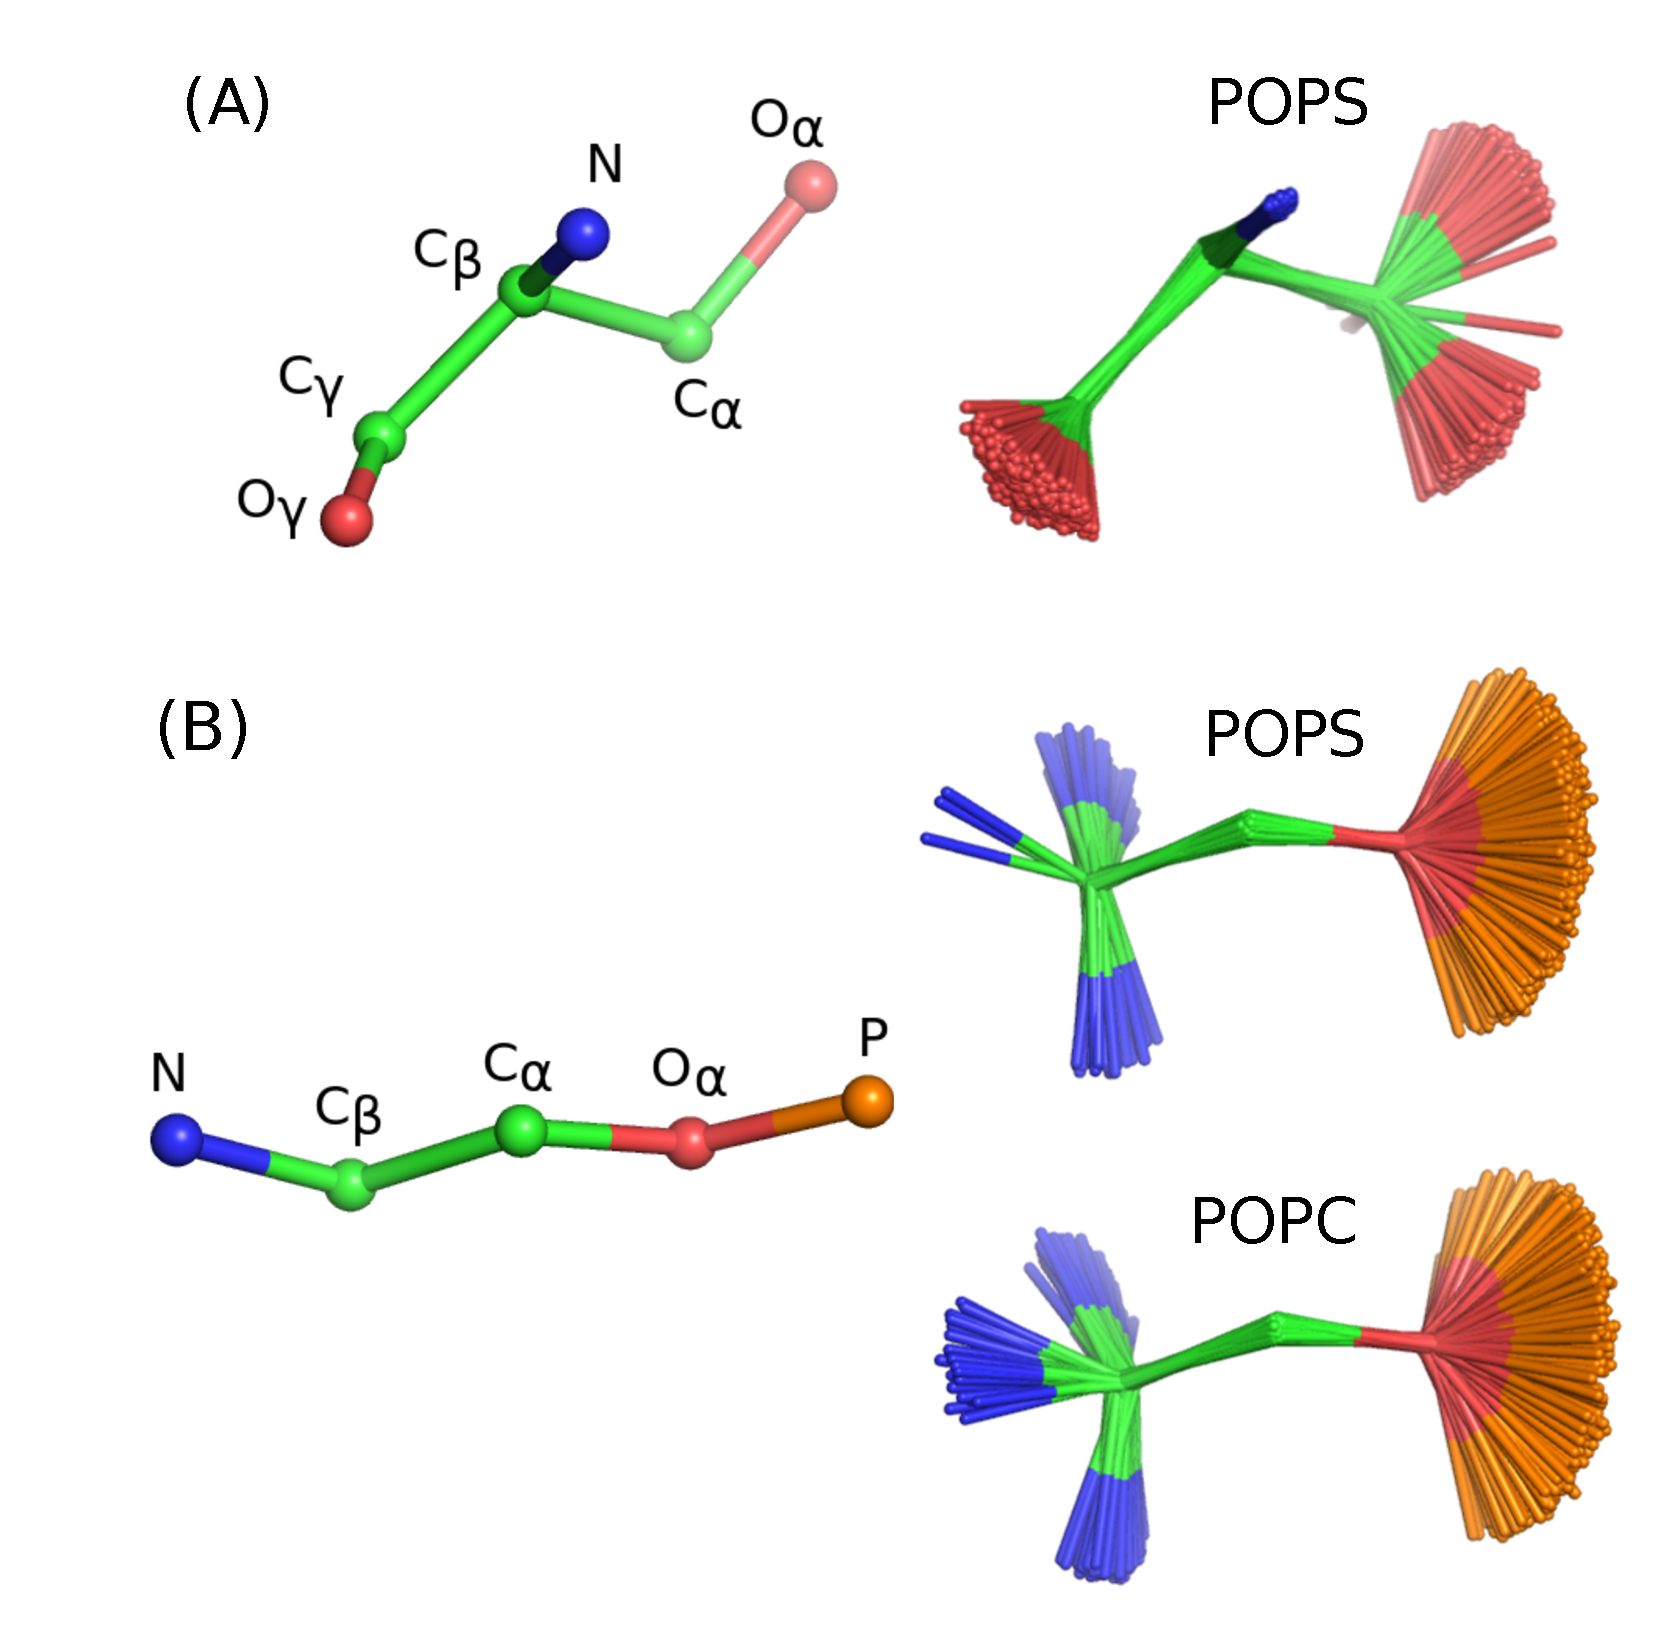
\includegraphics[width=9.0cm]{../Figs/structures.eps}
  \caption{\label{HGstructuresPSandPC}
    Overlayed snapshots from simulations conducted with CHARMM36---the force field producing the best agreement with experiments---demonstrate the conformational fluctuations
    in lipid headgroups.
    (A) Overlaying the C$_\gamma$, C$_\beta$, and C$_\alpha$ carbons demonstrates fluctuations around the O$_\gamma$-C$_\gamma$-C$_\beta$-C$_\alpha$, C$_\gamma$-C$_\beta$-C$_\alpha$-O$_\alpha$,
    and N-C$_\beta$-C$_\alpha$-O$_\alpha$ dihedrals of the PS headgroup.
    (B) Overlaying the C$_\beta$, C$_\alpha$, and O$_\alpha$ atoms demonstrates fluctuations around the N-C$_\beta$-C$_\alpha$-O$_\alpha$ and C$_\beta$-C$_\alpha$-O$_\alpha$-P
    dihedrals of the PS and PC headgroups. The trajectory used for CHARMM36 POPC is available at Ref.~\citenum{POPCcharmm36T303K}.}
\end{figure}

Interestingly, in the three models that best fit the experimental data,
the C$_\alpha$-C$_\beta$-C$_\gamma$-O$_\gamma$ dihedral angle distribution has a single peak around 120$^{\circ}$, while
the other models yield binodal distributions (Fig. \ref{dihedralsHG}).
The restricted motion is also visible in the sampled conformations (Figs.~\ref{HGstructuresPSandPC} (A) and \ref{HGandGLYstructuresPS}),
suggesting that the rotation of the carboxyl group is limited in the serine headgroup.
On the other hand, the C$_\beta$-C$_\alpha$-O$_\alpha$-P dihedral angle rotates relatively
freely between approximately 100$^{\circ}$ and 300$^{\circ}$ in the best three models (as seen also in Fig.~\ref{HGstructuresPSandPC} (B)),
while other models yield more restricted conformations (Fig. \ref{dihedralsHG}).

In simulations that have the best agreement with experiments (CHARMM36 and Slipids),
the N-C$_\beta$-C$_\alpha$-O$_\alpha$ dihedral exhibits a more asymmetric
angle distribution for PS than for PC headgroup (Figs.~\ref{HGstructuresPSandPC} (B) and \ref{dihedralsHGpc}),
which might reflect the increased rigidity proposed in the early experimental studies \cite{browning80,buldt81}.
Indeed, the characteristic conformations of the PS headgroup suggested here can be useful when interpreting experiments---however,
as none of the tested models fully reproduces the experimental order parameters, more accurate MD force fields are required to reveal the true conformational ensemble.

\subsection{Counterion binding and interactions between PC and PS headgroups}\label{ciBINDINGsection}

Membranes containing PS lipids are always accompanied with counterions that
modulate electrostatic interactions between the lipids and other biomolecules. MD simulations have suggested
that counterions reduce the area per lipid of PS bilayers compared to PC
bilayers~\cite{pandit02,mukhopadhyay04,pedersen06} by screening the repulsion between charged lipid headgroups.
We explored this by quantifying the counterion density profiles along the membrane normal, accompanied by the areas per lipid, see Fig.~\ref{NAdensPOPS}.
The force fields studied show significant differences in both binding affinity
and distribution of ions at the interface.
The experimental area per lipid (62.7~$\pm$~1.3~\AA$^2$) \cite{pan14} 
is reproduced only in GROMOS-CKP and in the MacRog simulation
with potassium counterions, while other models give considerably smaller values (Fig.~\ref{NAdensPOPS}).
However, the counterion binding and the concomitant electrostatic screening of the headgroup
repulsion does not fully explain the low area per molecule values
since the MacRog simulation, which has the strongest sodium binding
(the lowest concentrations in bulk water), gives the same area per molecule
as the CHARMM36-UA simulation, which has significantly weaker counterion binding
affinity. On the other hand, MacRog simulations with potassium produce a larger area per molecule (63~\AA$^2$) than
with sodium (53~\AA$^2$) in line with the weaker potassium binding affinity (Fig.~\ref{NAdensPOPS}).
The results are consistent with a previous study suggesting that the
low areas per molecule in PS lipid bilayers originate from the combination
of both the counterion binding and intermolecular interactions between lipid headgroups~\cite{petrache04}.

\begin{figure}[!htb]
  \centering
  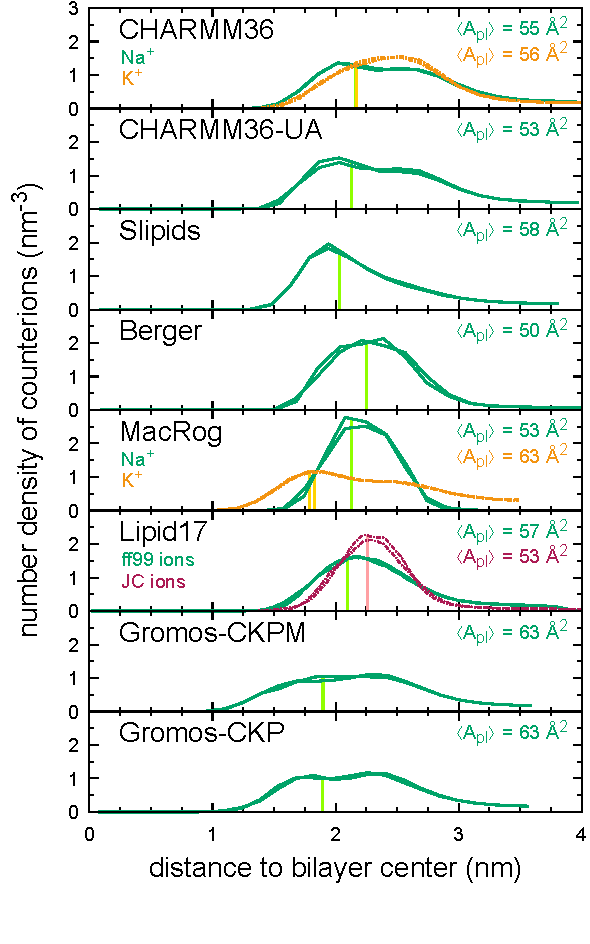
\includegraphics[width=9.0cm]{../Figs/NAdensPOPSformatted.pdf}
  \caption{\label{NAdensPOPS}
    Counterion density profiles along the membrane normal and areas per lipid (A$_{\rm pl}$)
    of POPS lipid bilayer from simulations with different force fields.
    The vertical green bars indicate the location of the phosphate density peak.
    The experimental area per lipid is~62.7~$\pm$~1.3~\AA$^2$~\cite{pan14}.
  }
\end{figure}




\begin{figure}[!tb]
  \centering
  \includegraphics[width=8.0cm]{../Figs/HGorderparametersPCvsPS.eps}
  \caption{\label{HGorderparametersPCvsPS}
    Changes of POPC headgroup order parameters with increasing amount of POPS in POPC:POPS mixtures at 298~K.
    Experimental values are from Ref. \citenum{scherer87}, with the signs measured in Ref.~\citenum{ferreira16}.
    The values from the CHARMM36 and GROMOS-CKP simulations with sodium are averages of two independent simulations and
    the error bar is given as the difference between the results divided by two.
  }\end{figure}

\begin{figure}[!tb]
  \centering
  \includegraphics[width=8.0cm]{../Figs/HGorderparametersPSvsPC.eps}
  \caption{\label{HGorderparametersPSvsPC}
    Modulation of POPS headgroup order parameters with increasing amount of POPC in POPC:POPS mixtures at 298~K.
    Experimental values with the signs are measured for pure POPS system in this work.
    The signs are assumed to be the same for the mixture and the values are from Ref. \citenum{roux90}.
    Because the experimental values of POPS in pure and mixed bilayers come from $^{13}$C NMR (this work) and $^2$H NMR (Ref. \citenum{roux90}), respectively,
    the error bars of 0.02 are used here \cite{botan15,ollila16}.
    The y-axis for the $\alpha$-carbon results of POPS (bottom) is shifted
    with the same value for both order parameters such that the lower order
    parameter value from pure POPS is at zero to correctly illustrate the significant forking.
    The values from CHARMM36 and GROMOS simulations are averages of two independent simulations and
    the error bars are given as the difference between the results divided by two. 
  }
\end{figure}



The experimentally observed modulation of headgroup order parameters
by increasing salt concentration (the molecular electrometer concept) has been previously used to evaluate the cation binding to zwitterionic PC bilayers in simulations \cite{catte16}.
Studying binding of cations to negatively charged lipid bilayers is less straighforward due to the presence of cationic
counterions (the lack of an ion-free reference state). The analysis is further complicated by the artificial aggregation of counterions
observed in some simulations (section \ref{mixtureTOadditionalCIs} in the SI).
Therefore, we evaluate here the amount of bound charge not by adding salt
(although this is discussed in the SI section \ref{mixtureTOadditionalCIs}),
but by studying the changes of the headgroup $S_{\rm CH}$ order parameters with increasing amount of
negatively charged lipids (and thus increasing amount of cationic counterions) in the bilayer.

Experimentally, the $S_{\rm{CH}}$ values of the $\alpha$ and $\beta$ headgroup carbons of POPC increase when negatively charged POPS lipids are incorporated in the bilayer 
(section \ref{HGorderparametersPCvsPEPSPGchol})~\cite{seelig87,scherer87}.
This is reproduced in the MacRog simulations with potassium counterions (Fig. \ref{HGorderparametersPCvsPS}),
which have the weakest binding affinity to POPS lipid bilayers (Fig.~\ref{NAdensPOPS}).
The CHARMM36, Berger and GROMOS-CKP simulations either exhibit no change or show a decrease
in either or both the POPC headgroup order parameters as the amount of POPS increases (Fig. \ref{HGorderparametersPCvsPS}).
Therein, the stronger counterion binding cancels
the effect of negatively charged headgroups and prevents the experimentally observed
increase of headgroup order parameters with growing amount of PS lipids.
Therefore, we suggest that the relatively weak binding of potassium
in the MacRog simulations (Fig. \ref{NAdensPOPS}) produces the most
realistic surface charge density in membranes containing PS lipids,
while the other tested models overestimate the counterion
binding affinity. The results are consistent with the behavior of headgroup order
parameters as a function of added counterions analyzed in section \ref{mixtureTOadditionalCIs}
in the SI.

The reduced forking of the POPS $\alpha$-carbon (Fig.~\ref{HGorderparametersPSvsPC})
together with other experimental results suggest that the PS headgroup structure becomes less rigid when diluted with
POPC~\cite{browning80,buldt81,roux90,roux91,scherer87}.
Unfortunately, none of the tested models correctly reproduce the modulation of POPS headgroup order
parameters with increasing amount of POPC in POPC:POPS mixtures (Fig. \ref{HGorderparametersPSvsPC}).
More accurate force fields are needed
to correctly describe the PC--PS headgroup interactions in MD simulations.

\subsection{Ca$^{2+}$ binding affinity to bilayers with negatively charged PS lipids}

\begin{figure*}[tbp]
  \centering
  \includegraphics[width=\textwidth]{../Figs/CHANGESwithCaClPS.eps}
  \caption{\label{changesWITHCaClPS}
   Variation of the POPC (left) and POPS (right) headgroup order parameters in a POPC:POPS (5:1) mixture
    as a function CaCl$_2$ concentration from experiments \cite{roux90} and from different force fields
    at 298~K (except the data for Berger are from a simulation of a POPC:POPS (4:1) mixture at 310~K \cite{ollila07a,melcrova16}). 
    The $S_\mathrm{CH}$ values from systems without calcium are set at the zero point of y-axes,
    except for the $\alpha$-carbon order parameters of POPS (bottom right), for which both $S^\alpha_\mathrm{CH}$ are shifted
    such that the lower $S^\alpha_\mathrm{CH}$ is zero without additional ions. This is to correctly illustrate
    the forking with different concentrations of calcium.
    Counterions were potassium in MacRog simulations, and sodium in Lipid14/17 Dang and CHARMM36 NBfix2 simulations.
    In CHARMM36 NBfix1, Lipid14/17 ff99, and Berger simulations with added calcium the lipid charge was neutralized with calcium, and monovalent counterions were not present;
    for these systems the $x$-axis shows [Ca$^{2+}$].
  }
\end{figure*}



Calcium binding affinity to membranes containing negatively charged PS lipids can be
experimentally quantified by measuring the PC lipid headgroup order parameters
from POPC:POPS (5:1) mixtures (see section~\ref{electrometerFORmixtures}),
where the measurement is not compromised by the dehydrated lipid--ion complexes and phase separation, and the bilayer remains uniform~\cite{feigenson86,mattai89,roux90,roux91}.
Despite the lack of an ion-free reference state
in the presence of negatively charged lipids, our simulations gave
coherent results for the POPC headgroup order parameters as a function of
CaCl$_2$ concentration in POPC:POPS (5:1) mixtures (Fig. \ref{changesWITHCaClPS}).
As expected from the previous study of pure PC lipid
bilayers \cite{catte16}, almost all the tested simulation models overestimated the
experimentally observed~\cite{roux90} decrease of the POPC headgroup $S_\mathrm{CH}$ upon increasing Ca$^{2+}$ concentration (Fig. \ref{changesWITHCaClPS}),
indicating too strong calcium binding affinity.
The sole exception was CHARMM36 when paired with the NBfix
corrections for calcium~\cite{kim16,han2018graph}; for these combinations, the modulation of order parameters was underestimated, 
indicating a weaker binding affinity than in experiments.
Notably, CHARMM36 with the NBfix corrections \cite{venable13,kim16} suggested similar binding affinities for
calcium and sodium to a POPC bilayer (see section \ref{CHARMMcalciumNBfix}), in contrast to experiments~\cite{cevc90,akutsu81,altenbach84}. This suggests that the calcium binding affinity
is underestimated in CHARMM36 when using the NBfix for calcium \cite{kim16,han2018graph}, but overestimated 
in all the other tested force fields. This is evident in the calcium density distributions, where almost all the Ca$^{2+}$ ions bind to the membrane interface in all models except CHARMM36 (Fig. \ref{CAdensPCPSmixture}).




\begin{figure}[tb]
  \centering
  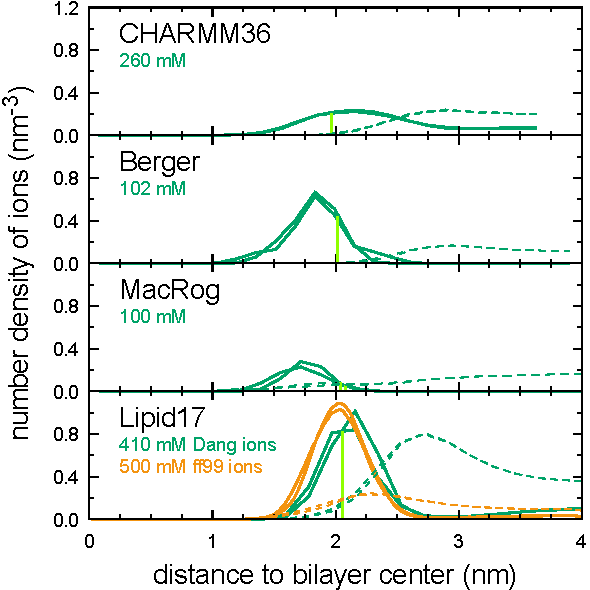
\includegraphics[width=9cm]{../Figs/CAdensPCPSmixtureLOWconsformatted.pdf}
  \caption{\label{CAdensPCPSmixture}
    Number density profiles of Ca$^{2+}$ (solid line) and Cl$^-$ (dashed line) from POPC:POPS (5:1) mixtures
    simulated with different force fields. The vertical green bars indicate the location of the phosphate density peak.
    The smallest simulated CaCl$_2$ concentrations are shown.
    The density profiles for all the simulated concentrations are given in SI figure \ref{CAdensPCPSmixtureALL}.
  }
\end{figure}


Experimentally, the POPS headgroup order parameters in POPC:POPS (5:1) mixtures
exhibit a strong response to small concentrations of CaCl$_2$, which saturates below 100~mM (Fig. \ref{changesWITHCaClPS}).
The $\beta$-carbon $S_\mathrm{CH}$ increases with added CaCl$_2$,
whereas the larger $\alpha$-carbon $S_\mathrm{CH}$ decreases. Moreover, a slight increase is observed in
the smaller $\alpha$-carbon $S_\mathrm{CH}$.
In simulations, all these responses were qualitatively correct only in CHARMM36.
In all force fields, even the qualitatively correct responses were much exaggerated---also in CHARMM36 that underestimated the Ca$^{2+}$ binding affinity---with
the sole exception of the larger $S^\alpha_\mathrm{CH}$, whose change CHARMM36 underestimated.
%All these changes were significantly overestimated in the tested simulation models---including CHARMM36 that underestimated the binding affinity.
Importantly, different force fields predicted qualitatively different behavior
for the two POPS $\alpha$-carbon order parameters as a function of added calcium:
Both order parameters decreased in Berger, but increased
in MacRog, whereas Lipid14/17 and CHARMM36 models exhibited more complex behaviors.
This is in contrast to the PC headgroup, where a
qualitatively correct response to bound ions is reproduced
by all simulation models, despite the significant discrepancies in the headgroup
structures observed in salt-free simulations~\cite{catte16}.
The divergent response of Berger may arise from the ring-like structures
observed in the headgroup region in this model (Fig. 6 in Ref. \citenum{mukhopadhyay04}).
Therefore, we conclude that
improvement of force fields is necessary to correctly capture the interactions between the
PS headgroup and calcium ions in MD simulations.

\section{Conclusions}

We used the headgroup C--H bond order parameters, $S_{\rm CH}$, and the open collaboration approach to evaluate the quality
of the headgroup structure and the ion binding affinity 
in available MD models of PS lipids.
The main advantage of using the $S_\mathrm{CH}$ is the direct connection they provide
between experiments and simulations: They can be measured accurately in experiments and calculated readily from simulations. 
This reduces the ambiguity in the interpretation of experiments.

First, we complemented the available experimental information \cite{browning80,roux90} by measuring the signs of the PS headgroup order parameters,
and then proceeded to compare MD simulation results from several force fields with the experimental data.
This revealed that none of the force fields
reproduce the PS headgroup order parameters within the experimental accuracy.
However, the best models captured essential differences between PS and PC, and
suggested characteristic conformations of PS headgroups.
Comparison to the experimentally observed order parameters in POPC:POPS (5:1) bilayers  at varying ion
concentrations \cite{roux90} then showed that the tested MD force fields
overestimate the cation binding affinity to these bilayers. There were two exceptions: 1) the MacRog force field with potassium counterions, which appeared to display a more realistic monovalent ion binding
affinity to PS-containing lipid bilayers than the other models; and 2) the CHARMM36 force field with the recently introduced
NBfix corrections for calcium \cite{kim16,han2018graph}, which underestimated the calcium binding affinity.
Importantly, the experimentally measured responses of the PS headgroup $S_\mathrm{CH}$ to bound calcium, as well as to dilution of the bilayer with zwitterionic PC lipids, were not
qualitatively reproduced in any of the tested force fields.
This is in contrast to previous results with PC lipids,
where MD force fields were seen to be at least in qualitative agreement with the experimentally measured headgroup $S_\mathrm{CH}$ responses to bound charge---even
though the headgroup structures themselves were
incorrect and the cation binding affinities were overestimated \cite{catte16}.
This underlines the dire need for more realistic MD force fields to study the biological function of PS lipids.

We expect our results to pave the way for the development of better PS force fields.
As the quality of the conformational ensembles can be evaluated
against the headgroup C--H order parameters, we hope that the $S_\mathrm{CH}$ will guide the development of
models that correctly reproduce the PS headgroup structures. For example, the ensembles we observed in the simulations
with the most realistic headgroup conformations (CHARMM36 and Slipids) do hint a direction for force
field improvement. The cation binding could be improved based on the experimental headgroup $S_\mathrm{CH}$
data from POPC:POPS (5:1) mixtures under different cation concentrations. Recent studies have shown that 
cation binding to bilayers with POPC and POPS lipids can be improved by implicit inclusion of electronic
polarizability using the electronic continuum correction (ECC) \cite{melcr18,ECCpops}, suggesting that
the electronic polarizability effects are important for lipid--ion interactions but polarizable force fields
may not be necessary to correctly capture ion binding to lipid bilayers.

\begin{suppinfo} 
 
%A listing of the contents of each file supplied as Supporting Information 
%should be included. For instructions on what should be included in the 
%Supporting Information as well as how to prepare this material for 
%publications, refer to the journal's Instructions for Authors. 
 
The following files are available free of charge. 
\begin{itemize} 
  \item SI.pdf: Additional simulation, experimental and methodological details, and further analysis. 
\end{itemize} 
 
\end{suppinfo} 


\begin{acknowledgement}
  HA acknowledges the Osk. Huttunen Foundation and the Finnish Academy of Science and Letters (Foundations' Post Doc Pool) for financial support.
  FFR acknowledges Tecnol\'{o}gico Nacional de M\'{e}xico Campus Zacatecas Occidente and
  Direcci\'{o}n General de Asuntos del Personal Acad\'{e}mico (DGAPA)
  Programa de Apoyo a Proyectos de Investigaci\'{o}n e Innovaci\'{o}n
  Tecnol\'{o}gica (PAPIIT) IG100416 for financial support and Cl\'{u}ster
  H\'{i}brido de Superc\'{o}mputo Xiuhcoatl-CINVESTAV and Miztli-Direcci\'{o}n de
  C\'{o}mputo y de Tecnolog\'{i}as de Informaci\'{o}n y Comunicaci\'{o}n (DGTIC)-Universidad Nacional Aut\'{o}noma de M\'{e}xico (UNAM) (Project
  LANCAD-UNAM-DGTIC-028) facilities for computing-time allocation.
  MJ acknowledges financial support from the Emil Aaltonen Foundation
  and CSC -- IT Center for Science for computational resources.
  JJM gratefully acknowledges financial support from the Carlsberg Foundation in the form of a postdoctoral fellowship while at the University of Chicago (grants CF15-0552, CF16-0639, and CF17-0783) and the research framework provided by the Research Computing Center at the University of Chicago.
  OHSO acknowledges financial support from Academy of Finland (315596),
  Integrated Structural Biology Research Infrastructure of
  Helsinki Institute of Life Science (Instruct-HiLIFE), and
  CSC -- IT Center for Science for computational resources.
  TJP wishes to acknowledge the use of the Iridis computing resources at the University of Southampton.
\end{acknowledgement}

%\newpage


% Create the reference section using BibTe
\bibliography{refsU.bib}

%\newpage
%\section{APPENDIX: The NMR results reported by Tiago Ferreira}

%\listoftodos

\end{document}
%
% ****** End of file aiptemplate.tex ******
